\documentclass[11pt]{article}
\pdfinfoomitdate=1
\pdftrailerid{}
\pdfsuppressptexinfo=-1
\ifdefined\pdfglyphtounicode
  \pdfgentounicode=1
  \pdfglyphtounicode{tfm:rm-lmr10/Omega}{03A9}
  \pdfglyphtounicode{tfm:lmmi10/mu}{03BC}
  \pdfglyphtounicode{tfm:lmmi8/mu}{03BC}
  \pdfglyphtounicode{tfm:lmsy10/openbullet}{2218}
  \pdfglyphtounicode{tfm:lmsy10/B}{212C}
  \pdfglyphtounicode{tfm:lmsy10/E}{2130}
  \pdfglyphtounicode{tfm:lmsy10/F}{2131}
  \pdfglyphtounicode{tfm:lmsy10/H}{210B}
  \pdfglyphtounicode{tfm:lmsy10/L}{2112}
  \pdfglyphtounicode{tfm:lmsy10/bardbl}{2016}
  \pdfglyphtounicode{tfm:lmsy10/backslash}{2216}
  \pdfglyphtounicode{tfm:lmsy8/B}{212C}
  \pdfglyphtounicode{tfm:lmsy8/E}{2130}
  \pdfglyphtounicode{tfm:lmsy8/H}{210B}
  \pdfglyphtounicode{tfm:lmsy8/backslash}{2216}
  \pdfglyphtounicode{tfm:msbm10/E}{1D53C}
  \pdfglyphtounicode{tfm:msbm10/F}{1D53D}
  \pdfglyphtounicode{tfm:msbm10/P}{2119}
  \pdfglyphtounicode{tfm:lmex10/parenleftbig}{0028}
  \pdfglyphtounicode{tfm:lmex10/parenrightbig}{0029}
  \pdfglyphtounicode{tfm:lmex10/bracketleftbig}{005B}
  \pdfglyphtounicode{tfm:lmex10/bracketrightbig}{005D}
  \pdfglyphtounicode{tfm:lmex10/vextenddouble}{2016}
  \pdfglyphtounicode{tfm:lmex10/parenleftBig}{0028}
  \pdfglyphtounicode{tfm:lmex10/parenrightBig}{0029}
  \pdfglyphtounicode{tfm:lmex10/parenleftbigg}{0028}
  \pdfglyphtounicode{tfm:lmex10/parenrightbigg}{0029}
  \pdfglyphtounicode{tfm:lmex10/bracketleftbigg}{005B}
  \pdfglyphtounicode{tfm:lmex10/bracketrightbigg}{005D}
  \pdfglyphtounicode{tfm:lmex10/ceilingleftbigg}{2308}
  \pdfglyphtounicode{tfm:lmex10/ceilingrightbigg}{2309}
  \pdfglyphtounicode{tfm:lmex10/parenleftBigg}{0028}
  \pdfglyphtounicode{tfm:lmex10/parenrightBigg}{0029}
  \pdfglyphtounicode{tfm:lmex10/bracketleftBigg}{005B}
  \pdfglyphtounicode{tfm:lmex10/bracketrightBigg}{005D}
  \pdfglyphtounicode{tfm:lmex10/parenlefttp}{239B}
  \pdfglyphtounicode{tfm:lmex10/parenrighttp}{239E}
  \pdfglyphtounicode{tfm:lmex10/parenleftbt}{239D}
  \pdfglyphtounicode{tfm:lmex10/parenrightbt}{23A0}
  \pdfglyphtounicode{tfm:lmex10/summationtext}{2211}
  \pdfglyphtounicode{tfm:lmex10/producttext}{220F}
  \pdfglyphtounicode{tfm:lmex10/summationdisplay}{2211}
  \pdfglyphtounicode{tfm:lmex10/productdisplay}{220F}
  \pdfglyphtounicode{tfm:lmex10/hatwide}{02C6}
  \pdfglyphtounicode{tfm:lmex10/hatwider}{02C6}
  \pdfglyphtounicode{tfm:lmex10/tildewide}{02DC}
  \pdfglyphtounicode{tfm:lmex10/radicalBig}{221A}
  \pdfglyphtounicode{tfm:rm-lmbx10/one}{1D7CF}
  \pdfglyphtounicode{tfm:eufm10/S}{1D516}
\fi

\usepackage[T1]{fontenc}
\usepackage{lmodern}
\usepackage[margin=1.05in]{geometry}
\usepackage{amsmath,amssymb,amsthm,mathtools}
\usepackage{microtype}
\usepackage{tikz}
\usetikzlibrary{arrows.meta,positioning,calc}
\usepackage{xcolor}
\definecolor{linkblue}{RGB}{20,69,103}
\PassOptionsToPackage{hyphens}{url}
\usepackage[colorlinks=true,linkcolor=linkblue,citecolor=linkblue,urlcolor=linkblue]{hyperref}
\hypersetup{pdftitle={Conditional permutations in a revealed switching environment},pdfauthor={OpenAI},bookmarksopen=true,bookmarksnumbered=true}
\newtheorem{theorem}{Theorem}[section]
\newtheorem{lemma}[theorem]{Lemma}
\newtheorem{proposition}[theorem]{Proposition}
\newtheorem{corollary}[theorem]{Corollary}
\theoremstyle{definition}\newtheorem{definition}[theorem]{Definition}
\theoremstyle{remark}\newtheorem{remark}[theorem]{Remark}
\newcommand{\TV}{\mathrm{TV}}
\newcommand{\op}{\mathrm{op}}
\newcommand{\HS}{\mathrm{HS}}
\newcommand{\E}{\mathbb E}
\newcommand{\one}{\mathbf1}
\newcommand{\id}{\mathrm{id}}
\DeclareMathOperator{\sgn}{sgn}
\DeclareMathOperator{\tr}{tr}
\numberwithin{equation}{section}
\title{Conditional permutations in a revealed switching environment}
\author{OpenAI}
\date{September 26, 2026}
\begin{document}
\maketitle
\begin{abstract}
Fix half the labels in a Thorp shuffle on $2^d$ positions and reveal their complete trajectories. We prove that, after an explicit absolute number of coordinate sweeps, the conditional permutation of the remaining labels approaches uniform in expected total variation as $d\to\infty$, uniformly in the initial layout. The resulting constructions give full-deck mixing in a constant multiple of $d$ physical shuffles.
\end{abstract}
\section{Introduction}

The random switches in a shuffle do more than move individual cards. They define a bijection between all starting and ending positions. If the paths of some cards are revealed, the other cards still undergo a random bijection, but its law depends on the revealed paths. We study when that entire conditional bijection becomes nearly uniform. This asks for information that is absent from a one-card mixing estimate: all remaining labels must be randomized together, after the surrounding motion has been observed.

The Thorp shuffle makes this distinction concrete. Split a deck into two equal halves, pair the cards in corresponding positions, and independently choose the order of each pair before interleaving them. For $n=2^d$ positions, undoing a deterministic rotation of the binary coordinates identifies successive shuffles with fair switches in the cyclic directions of the binary cube. A \emph{sweep} visits all $d$ directions once and costs $d$ physical shuffles. Each individual card is uniform after one sweep. The dependence among the routes of different cards remains substantial.

Write $U_m$ for uniform measure on the symmetric group $S_m$, and use total variation with its factor $1/2$. The mixing time $t_{\mathrm{mix}}(d)$ is the least number of physical shuffles at which the full-deck law is within $1/4$ of $U_n$ from every deterministic start. Fix $m=n/2$ outside labels. Given their full trajectories $\mathcal E$ through a time interval, list the unoccupied slots at each endpoint in increasing binary order. The switches map the initial free slots bijectively onto the final free slots; the resulting permutation of their indices has a conditional law $\nu_{\mathcal E}$ on $S_m$. Its definition uses the slot indices, independently of the order of the labels entering the interval. Section~\ref{sec:conditional} proves both this construction and the composition rule on consecutive intervals.

The main contribution is the information retained after the outside paths are revealed. An independent companion~\cite{optimal-order} gives full-deck mixing after $1600d$ physical shuffles. That conclusion concerns the unconditioned deck law; the theorem here controls the entire remaining assignment conditional on a path environment, with its own explicit time bound.

\begin{theorem}[Conditional permutation and full-deck mixing]\label{thm:methods}
Let $n=2^d$, and start the shuffle from any deterministic deck.
After $J(s_0+1)$ sweeps, where $s_0=400$ and $J=40000$, the conditional free-slot law defined above satisfies
\[
 \sup_{\text{initial layouts}}\E_{\mathcal E}
       \|\nu_{\mathcal E}-U_{n/2}\|_{\TV}\longrightarrow0
       \qquad(d\longrightarrow\infty).
\]
Consequently the full-deck law approaches uniform, uniformly in the starting deck, after $16\,040\,400d$ physical shuffles. For every integer $t\ge0$, after $t$ physical shuffles the full-deck distance from uniform is at least
$1-2^{tn/2}/n!$. Thus the full-deck mixing time is of order $d$.
\end{theorem}

The conditional conclusion says that the free-slot permutation is nearly independent of the revealed environment. Indeed, if $g$ is that permutation, then
\[
 \left\|\mathcal L(\mathcal E,g)
       -\mathcal L(\mathcal E)\otimes U_{n/2}\right\|_{\TV}
 =\E_{\mathcal E}\|\nu_{\mathcal E}-U_{n/2}\|_{\TV}.
\]
The equality follows by summing first over the environment and then over the permutation. For each fixed $\varepsilon>0$, Markov's inequality also shows that the probability of a conditional distance exceeding $\varepsilon$ tends to zero, uniformly in the initial layout. Rare path environments can nevertheless leave too few useful switches. The proof handles them by deleting a small amount of probability, with the loss measured under the actual outside-path law; it does not assume that a typical free set stays typical after further conditioning.

The first proof has three steps. We first mix any ordered half-deck in $400$ sweeps from every start. A two-copy calculation for a single sweep gives the exact collision kernel of a tagged free card. Splitting it into averages within large subcubes and fluctuations inside those subcubes produces a two-sweep contraction. Next, we alternate a preparation interval of $400$ sweeps with one active sweep. Truncating the preparation law gives domination by a uniform free set and an independent uniform slot permutation. The active sweep forces many coin agreements whenever two copies have many common endpoints. A symmetric-group character bound converts this into a normalized trace contraction. The preparation domination then turns that trace estimate into a matrix contraction which can be iterated while the outside paths continue to be revealed. Finally, we couple the outside half-decks and use the conditional result to couple the remaining labels.

The three subsequent constructions change a specific part of this mechanism. Their separate quantitative statements and time bounds are given with their proofs. Reset minorization uses an exact uniform component in a large marginal to create central relative-permutation increments. Its conditional collision identity gives uniformity even after all reset coins are revealed. Trajectory overlays preserve the true shuffle law by adding predictable independent switches to a base trajectory system. They first randomize one group of indices and then use three rounds on transverse partitions; a local limit estimate for contingency tables completes that route. The last construction conditions on the unlabelled occupancy history of two colors. Given that history, the two internal half-permutations are independent. Conditional list estimates and a signed-tabloid transfer then control a two-block Fourier matrix. These are different conditional objects, and each construction includes its own mass and independence argument.

The shuffle originates in Thorp's study of shuffling and Faro~\cite{thorp}. Morris proved an $O(d^{44})$ bound for power-of-two decks~\cite{morris44}; Montenegro and Tetali gave the intermediate $O(d^{29})$ bound~\cite[Theorems~6.14--6.15]{montenegro-tetali2006}. Morris subsequently obtained an $O((\log n)^4)$ bound for every even deck size~\cite{morris4} and an $O(d^3)$ bound for $n=2^d$~\cite{morris3}.

For partial permutations, Czumaj and V\"ocking proved that the endpoint positions of any prescribed $\lfloor cn\rfloor$ cards mix in $O(d^2)$ physical Thorp shuffles, for each fixed $0<c<1$ and $n=2^d$~\cite{czumaj-vocking2014}. Morris's chameleon analysis already studies a tagged card conditional on an occupancy history in an auxiliary zigzag shuffle~\cite[preprint, Section~4, Lemma~3]{morris44}. Partial permutation laws also appear in the enciphering work of Morris, Rogaway and Stegers~\cite[Theorem~1 and Lemma~2, proved in Appendix~A]{mrs}. Hoang, Morris and Rogaway use conditional squared energies and sequential total-variation comparison in their analysis of swap-or-not~\cite[Section~3]{hmr2014}. Their random-key chain differs from the deterministic coordinate schedule here. Our conditional permutation estimates require the additional bijection, truncation and character arguments developed below.

The character input is the uniform Larsen--Shalev estimate~\cite[Theorem~1.1]{larsen-shalev2008}, in the precise fixed-slack formulation recorded by Keller, Lifshitz and Sheinfeld~\cite[Definition~2.1 and Theorem~2.2]{keller-lifshitz-sheinfeld2024}. Standard branching, Schur orthogonality and hook-length formulas are used in the conventions of~\cite{sagan,etingof}. Lemmas~\ref{lem:character-fixed-points} and~\ref{lem:degree-sum} collect the character consequences and an elementary reciprocal-square degree estimate used across the constructions. The latter is a special case of the general summability theorem of Liebeck and Shalev~\cite[Theorem~2.6]{liebeck-shalev2004}.

Sections~\ref{sec:conditional}--\ref{sec:burn-completion} give the entire first route. Sections~\ref{special:reset} and~\ref{special:overlay} give the reset and overlay constructions. Section~\ref{sec:two-halves} identifies precisely the conditional path theorem and the abstract signed-tabloid transfer used in the two-half construction. The companion on conditional coordinate sweeps~\cite{conditional-sweeps} studies prescribed trajectories in a different, near-uniform line model. It retains a falling-factorial potential through the conditional moment induction; with no prescribed paths, the resulting dimension estimate is then transferred analytically to binary sweeps. Its theorem is not an input to the present kernels.

\section{From revealed paths to a permutation kernel}\label{sec:conditional}

We first specify the information being conditioned on and prove that the unobserved randomness acts on the whole free assignment. The distinction between a positional bijection and the labels carried by that bijection will matter when preparation intervals are repeated.

Identify the positions with $V=\mathbb F_2^d$, ordered lexicographically. Permutations send labels to positions, and $(gh)(x)=g(h(x))$. Put
\[
 R(x_1,\ldots,x_d)=(x_2,\ldots,x_d,x_1).
\]
One physical shuffle is $RS$, where $S$ independently fixes or exchanges each pair $\{x,x+e_1\}$. If $Y_t$ is the physical permutation and $X_t=R^{-t}Y_t$, then
\[
 X_{t+1}=R^{-t}S_{t+1}R^tX_t.
\]
Thus $X_t$ uses independent fair matching switches in directions $1,\ldots,d$ cyclically. A layer means one such update; a sweep consists of $d$ consecutive layers containing all directions. At sweep boundaries $X_t=Y_t$. All interval lengths used below end at such boundaries. Uniform measure on the full group, and on every ordered-injection space, is invariant under each layer.

\begin{lemma}[Conditional slot bijections]\label{lem:slot-kernel}
Fix a deterministic starting layout and a set of outside labels. For any feasible specification $e$ of their paths through a finite interval, conditional on $e$ all switch values on edges incident to an outside card are fixed, and all other switch values are independent fair bits. Let $F_s$ be the set of free positions at boundary $s$, and let $m=|F_s|$. Write $\iota_s:[m]\to F_s$ for the increasing bijection. Every completion of the unexposed bits induces a bijection $T_e:F_0\to F_T$, hence a permutation
\[
 g_e=\iota_T^{-1}T_e\iota_0\in S_m.
\]
Its conditional law depends on the outside paths and positions, but not on the incoming assignment of free labels. On consecutive intervals the corresponding permutations multiply with later intervals on the left. Conditional on all the outside paths, their remaining switch arrays are independent, so their conditional laws compose by convolution.
\end{lemma}
\begin{proof}
At a given layer, a specified outside path records both the incoming and outgoing endpoint of its matching edge and thereby fixes that edge's coin. If two outside cards meet, feasibility makes their requirements agree. Conversely, prescribing those values forces the outside paths: induction on the layer determines their positions regardless of all other switch values. The path event is exactly a cylinder in the independent time-edge coin array. Conditioning therefore leaves every unprescribed time-edge coordinate independent and fair, including coordinates earlier than a future prescribed path segment.

At a layer there are three cases. An outside--outside edge has no free slot. An outside--free edge has one free input and one free output, and the prescribed coin maps the former to the latter. A free--free edge has two free inputs and outputs, and its unexposed coin chooses the identity or transposition. These maps are bijections between the free input and output sets. Their composition is $T_e$. Relabelling the free cards changes neither the cylinder event nor these maps. If an incoming label assignment is a bijection $a:[m]\to\mathcal L$ from the slot indices to the free-label set $\mathcal L$, the outgoing assignment is $a\circ g_e^{-1}$. Consequently a uniform $g_e$ gives a uniform assignment, whatever $a$ is.

At an intermediate boundary the same increasing map $\iota_s$ is used as the terminal index map of one interval and the initial index map of the next. These maps cancel in the product, giving the stated multiplication order. The unexposed time-edge coordinates of disjoint intervals are disjoint. The cylinder description proves their conditional independence even when all outside paths, including future ones, have been revealed. Each factor law is the one obtained by conditioning only on that interval's outside paths and starting outside layout.
\end{proof}

The lemma extends the elementary path-cylinder observation to a law on $S_m$. It does not assert that this law is already uniform. In particular, its one-card marginals need not determine it. The next two sections supply the contraction of the full law.

\begin{figure}[ht]
\centering
\begin{tikzpicture}[>=Stealth, node distance=18mm]
\node (a) {$[m]$};
\node[right=24mm of a] (f) {$F_0$};
\node[right=30mm of f] (g) {$F_T$};
\node[right=24mm of g] (b) {$[m]$};
\draw[->] (a)-- node[above] {$\iota_0$} (f);
\draw[->] (f)-- node[above] {$T_e$} (g);
\draw[->] (g)-- node[above] {$\iota_T^{-1}$} (b);
\draw[->] (a.south) to[out=-45,in=-135] node[below] {$g_e=\iota_T^{-1}T_e\iota_0$} (b.south);
\end{tikzpicture}
\caption{A fixed revealed path environment determines the free sets. Unexposed switches determine a random bijection between them. Increasing slot indices turn this bijection into a permutation on one fixed group, so consecutive kernels can be multiplied.}
\label{fig:slots}
\end{figure}

For one tracked free card, Lemma~\ref{lem:slot-kernel} gives a simpler linear evolution. Its conditional masses are averaged across a free--free edge and transported across a mixed edge. The uniform vector on the free slots follows exactly the same transport. A signed difference from uniform therefore has sum zero and nonincreasing Euclidean norm. This linear evolution is adapted to the progressively revealed paths, despite being a formula for the law conditional on their entire final specification: later prescribed coins do not reveal earlier unexposed ones.

We will also use uniqueness of an individual path through a single sweep. Just before direction $i$ is updated, the earlier coordinates equal the card's terminal coordinates and the later coordinates equal its initial coordinates. Thus the initial and terminal positions determine every intermediate position. This statement holds for any cyclic phase and either order of the coordinates.

Finally, the support bound in Theorem~\ref{thm:methods} needs no conditioning. There are at most $2^{tn/2}$ coin strings in $t$ physical shuffles. Their support has uniform mass at most $2^{tn/2}/n!$, proving the bound. In particular distance at most $1/4$ requires
\[
 t\ge\left\lceil\frac2n\log_2\frac{3n!}{4}\right\rceil
       =2d-O(1).
\]
For comparison with the lower constants in the separate constructions, the elementary inequality $n!\ge(n/2)^{n/2}$ also gives distance at least $1-2^{-n/2}$ whenever $t\le d-2$. Stirling's bound $\log(n!)\ge n\log n-O(n)$ gives distance tending to one uniformly for $t\le d$. In particular the weaker lower constants $d/2$, $d-1$ and $d$ used by those constructions follow from this same support calculation.

Changing the initial deck translates a permutation law, so its distance from uniform is unchanged. Mixing exists in each fixed dimension: one sweep has positive probability of being the identity or any specified cube-edge transposition, and those transpositions generate $S_n$. Identity sweeps pad finite products to a common length, giving a positive uniform minorization for a sufficiently long sweep block.

\section{Preparing an ordered half-deck}\label{sec:preparation}

Throughout this section put $m=n/2$. Our first task is to randomize any specified ordered half-deck from a deterministic start in $400$ sweeps, uniformly in its starting positions. The conditional-bijection construction of Lemma~\ref{lem:slot-kernel} supplies its one-card transition matrices. We first establish the complementary one-sweep estimates that will make these matrices contract over pairs of sweeps.

Consider one sweep with blocked positions \(E\) at its start, \(r=|E|\le m\). For the random blocked paths let \(E'\) be the end positions and \(Q\) the conditional single-free-card transition matrix (rows in \(E^c\), columns in \((E')^c\)). It is doubly stochastic between these two sets, since the conditional moves are random bijections. Vectors of probabilities or their differences will be row vectors, with the ordinary Euclidean norm. In particular \(\|uQ\|\le\|u\|\), by convexity of the square applied in each column and then the row sums. Put \(A_E=\mathbb E[QQ^\top]\), the expectation over these paths from the fixed blocked start. Its entry at \(x,y\in E^c\) is the probability two copies starting at \(x,y\), run independently conditional on the common blocked paths, finish at the same position (averaging also over the paths). It is symmetric and a contraction, as is \(QQ^\top\).

Let \(h=\lfloor d/2\rfloor\), and call the blocks specified by bits \(>h\) the coarse blocks (size \(2^h\)). For a free-slot vector \(u\) write \(u_{\rm c}\) for its orthogonal projection obtained by averaging over free slots within each such block (ignoring empty ones). Call a blocked set good if its fraction in every coarse block is at most \(3/4\). Set \(q=7/8\) and
\[
 \epsilon_n=n\left(\frac{3/2}{2^{3/4}}\right)^{2^h}.
\]

We use a two-sweep mechanism. From a balanced blocked set, one sweep contracts fluctuations within large subcubes. It may leave averages that differ between subcubes, but the same sweep makes the expected energy of those output averages small. Combining the two estimates in the next sweep will contract the whole vector. The next lemma gives the two estimates and the probability of an unbalanced output.

\begin{lemma}[Coarse-block estimates]\label{lem:coarse-block-estimates}
For the one-sweep matrix $Q$ defined above and every free-slot row vector $u$, a good starting blocked set $E$ satisfies
\begin{equation}
 \mathbb E\|uQ\|^2=u A_E u^\top
 \le \|u_{\rm c}\|^2+q^{d-h}\|u\|^2. \label{special:burn-active:eq:2}
\end{equation}
For every starting blocked set $E$ with $|E|\le n/2$, the ending set satisfies
\begin{equation}
 \mathbb P(E'\text{ not good})\le
 \epsilon_n. \label{special:burn-active:eq:3}
\end{equation}
If $u$ has sum zero, then its coarse part on the ending free slots satisfies
\begin{equation}
 \mathbb E\|(uQ)_{\rm c}\|^2\le (4\cdot 2^{-h}+\epsilon_n)\|u\|^2. \label{special:burn-active:eq:4}
\end{equation}
\end{lemma}
\begin{proof}
Write \(p_k(x)\) for the initial blocked fraction in the block of size \(2^{k-1}\) having bits \(>k\) equal to those of \(x\) and bit \(k\) opposite to that of \(x\), and set \(q_k(x)=(1+p_k(x))/2\). Let \(j\) be the largest coordinate where \(x,y\) differ, or \(0\) if they coincide. We claim
\begin{equation}
 A_E(x,y)=2^{-j}\prod_{k=j+1}^d q_k(x). \label{special:burn-active:eq:1}
\end{equation}
For the two-copy experiment averaged over paths, we can generate the blocked motion with independent switch coins, use these moves for the copies where an edge is incident to a blocked card, and use two fresh independent arrays of switch coins (one per copy) on free-free edges. Whenever the copies are at different positions before a stage, their two new bits at that stage are independent uniform bits given the history up to then: for different edges the coins used are independent, and if the edge is the same, both its slots must be free and the copies use independent coins. Up to and including stage \(j\) the pre-switch positions are different, due to bit \(j\) if \(j>0\). Thus the probability of matching the first \(j\) new bits is \(2^{-j}\), after which they are at the same position on that event. A mismatch in any updated bit persists to the end of the sweep.

For \(k>j\), given they matched the new bits through stage \(k-1\) (so are now together), they stay together for sure if the neighbor slot is blocked and with probability \(1/2\) otherwise. Here the probability the neighbor is blocked, given this matching so far and their current common prefix, is \(p_k(x)\). To see this, before stage \(k\) both copies have evolved in the block with bits \(\ge k\) equal to those of \(x\). Their motion and the event of matching so far only use coin arrays in that block. In the neighboring block (bit \(k\) opposite), independently, the blocked configuration has evolved for \(k-1\) stages within the block; each initial blocked card there has uniform marginal position in it, since its successive new bits are conditionally fair. Thus the blocked probability at the slot matching the copies' prefix is the stated fraction. This independence uses a fixed initial \(E\) and disjoint switches of the blocks prior to stage \(k\). Multiplying the stay-together probabilities proves \eqref{special:burn-active:eq:1}, including for \(j=0\).

To prove \eqref{special:burn-active:eq:2}, note that \eqref{special:burn-active:eq:1} is constant between any two fixed distinct coarse blocks. Within the block of \(x\), its row sum equals \(\prod_{k=h+1}^d q_k(x)\): for \(1\le j\le h\) there are \(2^{j-1}(1-p_j(x))\) free \(y\)'s with that last difference, contributing \((1-q_j(x))\prod_{k>j}q_k(x)\), which telescope together with the diagonal term. This row sum is constant for \(x\) in the block, and is at most \(q^{d-h}\) when \(E\) is good since the blocks defining \(p_k\) for \(k>h\) are unions of coarse blocks. The coarse-constant subspace is invariant under \(A_E\) by the constants and row sums just noted; on it we use contraction. On its orthogonal complement the between-block entries contribute zero, and the symmetric within-block matrices have norm at most their maximum row sum (nonnegative entries). By symmetry there is no cross term between the two subspaces. This proves \eqref{special:burn-active:eq:2}; without goodness we still have contraction.

We also bound the expected coarse part at the \emph{output}, with the same choice of coarse coordinates for use in the next sweep. Let \(H(x,y)\) be the probability in the two-copy experiment of equal bits \(>h\) at the output, and \(H_{\rm pre}(x,y)\) the probability of equal bits \(1,\ldots,h\). Then, with the all-ones matrix denoted by \({\bf 1}{\bf 1}^\top\),
\[
 H=2^{-(d-h)}({\bf 1}{\bf 1}^\top-H_{\rm pre})+A_E .
\]
If the first \(h\) bits mismatch, the copies remain at distinct positions, so the remaining new bits match with probability \(2^{-(d-h)}\) by the fresh-bit observation for distinct positions. If the first \(h\) match, also matching the rest means an end collision. Moreover \(H_{\rm pre}\) is positive semidefinite: conditional on the blocked paths the equality probabilities form a Gram matrix of the transition probabilities aggregated by output prefix, and we average this matrix. Consequently for \(u\) of sum zero, the expected sum over coarse output blocks of the squared sums of \(uQ\) in them is \(u H u^\top\le u A_E u^\top\le\|u\|^2\).

We prove directly the needed negative-dependence inequality. It is a restricted form of the preservation of negative dependence under partial symmetrization studied by Borcea, Br\"and\'en and Liggett~\cite[Theorems~4.9 and~4.20]{bbl2009}. The blocked-slot indicators throughout the switches satisfy: for any set of slots the probability all are blocked is bounded by the product of their marginal probabilities. It holds initially (deterministic); a single fair swap preserves it. For a test set containing one of the two slots, average the two old bounds, and for one containing both, use that the product of their marginals can only increase when both marginals are replaced by their average. Disjoint simultaneous swaps can be processed one at a time. After a sweep all marginals are \(r/n\) by single-card uniformity. For the number \(B\) blocked in a given coarse block, expanding the product of \(1+\)indicator over it thus gives \(\mathbb E 2^B\le(1+r/n)^{2^h}\); Markov's inequality and the union bound give \eqref{special:burn-active:eq:3}.

On good output the squared block sums are divided by block free-slot counts at least \(2^h/4\) to form the squared norm (use the unconditional numerator bound), and on bad output the norm is at most \(\|u\|\) by contraction. Together with \eqref{special:burn-active:eq:3}, this proves \eqref{special:burn-active:eq:4}.

\end{proof}

\begin{proposition}[Uniform half-deck preparation]\label{prop:half-preparation}
For all sufficiently large $d$, every ordered list of $k\le n/2$ distinct labels, from every deterministic starting layout, has endpoint law within $n^{-3}$ in total variation of uniform ordered distinct positions after $400$ sweeps.
\end{proposition}
\begin{proof}
Fix at most $m$ blocked cards and track one specified free card over sweeps, starting deterministically, and let \(u_s\) be its law conditional on the blocked paths up through sweep \(s\), minus uniform on the then free slots. Given those paths, the next blocked paths are fresh from the then layout, and on revealing them \(u_{s+1}=u_s Q\) for their conditional matrix; future blocked paths supply no information on the unused free coins of the past, and the uniform vectors are carried to uniform vectors. In particular there is pathwise norm contraction. Write \(a_s=\mathbb E\|u_s\|^2\), with \(a_0\le1\). For \(s\ge1\), the mean squared coarse part of \(u_s\) is bounded by \((4\cdot 2^{-h}+\epsilon_n)a_{s-1}\) by \eqref{special:burn-active:eq:4} given the paths through the previous sweep. Also \(\mathbb E[{\bf 1}_{\{\text{bad after }s\}}\|u_s\|^2]\le\epsilon_n a_{s-1}\) by pathwise contraction and \eqref{special:burn-active:eq:3} given the previous paths. Applying \eqref{special:burn-active:eq:2} for the next sweep on good starts and contraction otherwise, we get
\[
 a_{s+1}\le q^{d-h}a_s+(4\cdot 2^{-h}+2\epsilon_n)a_{s-1}
 \le n^{-1/20} a_{s-1}
\]
for all sufficiently large \(d\). Here \(a_s\le a_{s-1}\), \(\epsilon_n\) decays faster than any inverse power of \(n\), and \(\log_2(8/7)/2>1/20\). Take the fixed length \(s_0=400\) sweeps; iterating with sweep index jumping by two gives \(a_{s_0}\le n^{-10}\).

It follows that for any ordered list of \(k\le m\) cards from any fixed start,
\begin{equation}
 d_{\rm TV}(\text{law of their positions after }s_0\text{ sweeps},
            \text{uniform ordered distinct positions})\le\delta_n:=n^{-3} \label{special:burn-active:eq:5}
\end{equation}
for large \(d\). For each next card condition first on the \emph{paths} of the previous cards on the list, taking them as the blocked cards above. The mean total variation deviation from uniform on the remaining end slots is at most \(\sqrt{n a_{s_0}}/2\) by Cauchy-Schwarz. Conditioning instead only on the previous endpoints can only lower this averaged bound, by mixtures with the same uniform comparison given those endpoints. Sum these next-card bounds to bound the joint total variation: one can interpolate laws by taking an initial part of the list with its actual endpoint law and filling the rest uniformly without replacement. Consecutive such laws differ in total variation by at most the averaged next-card deviation (with previous endpoints actual). Since \(k\sqrt{n\cdot n^{-10}}/2\le \delta_n\), this gives \eqref{special:burn-active:eq:5}. This sequential total-variation comparison also appears in Morris's exclusion-process analysis~\cite[Lemma~12]{morris-exclusion2006}.

\end{proof}

\section{Preparation and active sweeps}\label{sec:burn}

Now designate \(m\) labels as outside cards, leaving \(m\) free cards, from any deterministic layout at a sweep boundary. We will bound the expected distance of the free-slot kernel from uniform on \(S_m\), conditional on all outside paths. Index the free slots increasingly at each boundary. By Lemma~\ref{lem:slot-kernel}, interval kernels compose by convolution, with later increments on the left, independently of the incoming free-label assignment. Each factor is computed from that interval's outside paths and starting outside layout, even when the entire outside history is revealed.

Partition the time here into chunks, each a preparation interval of \(s_0\) sweeps and then an active interval of one sweep. A subprobability is a nonnegative measure of total mass at most one. The two intervals have different tasks. After averaging over the actual preparation paths, we need joint domination by a uniform endpoint free set and an independent uniform slot permutation; this will permit a Schur conjugation average. During the active sweep, we need enough fresh coin constraints that agreement of many endpoints is unlikely. We achieve both by restricting or downweighting outcomes, obtaining conditional subprobability laws whose mean missing mass will be restored at the end.

\subsection{Truncating the preparation interval} Given the chunk's starting layout with free set \(z_0\), consider the ordered endpoint injection \(y\) at the end of the preparation interval of fictitious free labels placed canonically in the free slots at its start. Let \(p(y)\) be its probability \emph{without} conditioning on paths, from this start. Equivalently \(y\) encodes the endpoint free set \(z\) and the preparation permutation \(g\) on the canonical indices. Write \(u_*=(\binom{n}{m}m!)^{-1}\) for the uniform injection probability. Weight the preparation outcomes by \(\min(1,u_*/p(y))\) (use 1 at \(p(y)=0\)), using \(y\) of this interval's canonical increment, not the endpoints of labels carried in from prior chunks. Denote the resulting subprobability on \(g\) conditional on preparation outside paths \(e\) by \(\widetilde\nu_b^e\). Since \(z=z(e)\) is determined by those paths,
\begin{equation}
 \mathbb E_e\big[{\bf 1}_{\{z(e)=z\}}\widetilde\nu_b^e(g)\big]
 =\min(p(y),u_*)\le u_* \qquad\text{for each }(z,g). \label{special:burn-active:eq:6}
\end{equation}
Thus the retained joint measure averaged over paths is dominated by the law of uniform \(z\) and independent uniform \(g\). By \eqref{special:burn-active:eq:5} the expected removed mass is at most \(\delta_n\). Also the unweighted marginal of \(z\) is within \(\delta_n\) of uniform.

\subsection{Active truncation} For each free carrier (card considered from its slot at the start of the active sweep), count the stages of this sweep at which it is on an edge with two free slots. Call the carrier poor if this count is less than \(d/4\). Retain the active trajectory if at most
\[
 L=n^{1-1/40}
\]
free carriers are poor, dropping it otherwise. This criterion does not depend on their incoming labeling. With active outside paths \(e'\), write \(\widetilde\nu_a^{e'}\) for the conditional subprobability law of the active permutation.

At a uniform start set \(z\) independent of the fresh switches, the probability of dropping is at most \(n^{-1/40}\) for large \(d\). In fact for any full sweep switch realization form the meeting graph on the \(n\) initial slots, joining two whose carriers occupy the two slots of the same switch at some stage. It has \(d\) distinct neighbors per slot: after such a meeting at stage \(i\) the two differ in bit \(i\) and keep differing there through the sweep, preventing any later meeting in it. The graph does not use \(z\). Given a particular slot is in the uniform free set, for its \(d\) neighbors the probability any \(k\) specified ones are all outside is at most \((m/(n-1))^k\) (sampling without replacement). As in \eqref{special:burn-active:eq:3}, the probability of having more than \(3d/4\) outside neighbors is at most
\[
 (1+m/(n-1))^d 2^{-3d/4}\le n^{-1/20}
\]
for large \(d\) (the limiting \(\log_2(3/2)<7/10\)). This bounds the poor probability for that free slot. The expected number poor is thus at most \(m n^{-1/20}\); apply Markov's inequality to obtain the dropping bound. Generating full switches here computes exactly the expected removed conditional mass when averaging over the outside paths and the free switches. This path-averaged loss as a function of the active starting layout depends only on its free set (relabeling the outside has no effect). Thus from the end of the unweighted preparation interval its expectation is at most \(n^{-1/40}+\delta_n\), for any start of the chunk.

The active subprobability has zero sign transform:
\[
 \sum_g \widetilde\nu_a^{e'}(g)\operatorname{sgn}(g)=0.
\]
The free-free edge sets are determined by \(e'\). If there are none, no trajectory is retained for large \(d\) (\(m>L\)). Otherwise flip the free coin on one fixed free-free edge at the last stage having any. The counts for the carriers are unchanged (no further free-free stages), retention is invariant, and this probability-preserving involution changes the endpoint parity by exchanging the endpoints of the two carriers there.

\subsection{Trace estimate for an active interval}

Use unitary complex irreducible representations \(\rho\) of \(S_m\), writing the transform of a measure as \(F=\sum_g \nu(g)\rho(g)\). Denote by \(D\) the dimension and \(\chi\) the (unnormalized) character. We use the ordinary trace, with $\|B\|_{\HS}^2=\operatorname{tr}(B^*B)$. Write \(F_a\) for the transform of \(\widetilde\nu_a^{e'}\), and put
\[
 A(z)=\mathbb E_{e'}[F_a^*F_a\mid\text{active start with free set } z],
 \qquad b_\rho=\mathbb E_{z\ {\rm uniform}}\frac{\operatorname{tr} A(z)}{D}.
\]
The expectation defining \(A(z)\) is the same for any outside labeling of the other slots: such a relabeling just bijects outside paths with the same constraints on switch moves and the same probabilities and free kernels. For the sign representation \(F_a=0\). We treat \(D>1\) next.
The representation-theoretic background used here is recalled in~\cite{sagan,etingof}.

For the trace, conditional on \(e'\), take two independently generated free switch realizations \(X,Y\); letting \(g_X,g_Y\) be the resulting permutations, expansion gives \(\operatorname{tr}(F_a^*F_a)\) equal to the conditional average of \(\chi(g_X^{-1}g_Y)\) times the indicators that both are retained. Let \(f\) be the number of fixed points of \(g_X^{-1}g_Y\). Given a retained \(X\), for any \(a\) specified free starting indices to be fixed, their carriers must have the same paths in \(Y\) as in \(X\), by single-sweep path uniqueness from endpoints. At least \(a-L\) of them are not poor in \(X\), so they jointly visit at least \(d(a-L)/8\) distinct free-free switches (at most two carriers per switch). The coins there in \(Y\) would all have to match, and they are independent fair coins conditional on \(e'\) and \(X\). By a union bound, with \(\beta=1/100\) and for integers \(n^{1-\beta}\le a\le m\),
\begin{equation}
 \mathbb P(f\ge a,\ X,Y\text{ retained}\mid e')
 \le \binom{m}{a} 2^{-d(a-L)/8}
 \le n^{-a/32} \label{special:burn-active:eq:7}
\end{equation}
for large \(d\), since \(L\le a/2\) and \((em/a)^a\le n^{2\beta a}\) (here \(e\) in \(em/a\) is the base of natural logarithms).

The endpoint-agreement estimate must now be converted into a character estimate. We record the two bounds used here and in the reset and overlay constructions.

\begin{lemma}[Characters and fixed points]\label{lem:character-fixed-points}\label{input:character}
Fix $0<\delta<1/4$. For all sufficiently large integers $r$, every irreducible character $\chi$ of $S_r$, of degree $D=\chi(1)$, and every $\sigma\in S_r$ with $f$ fixed points satisfy
\begin{align}
 f\le r^{1-4\delta}&\quad\Longrightarrow\quad
       \frac{|\chi(\sigma)|}{D}\le D^{-\delta},\label{eq:character-small-fixed}\\
 \frac{|\chi(\sigma)|}{D}&\le D^{-\delta}r^{\delta f}.\label{eq:character-all-fixed}
\end{align}
The threshold for $r$ depends only on $\delta$.
\end{lemma}
\begin{proof}
We use the uniform Larsen--Shalev bound~\cite[Theorem~1.1]{larsen-shalev2008}, in the fixed-slack formulation of~\cite[Definition~2.1 and Theorem~2.2]{keller-lifshitz-sheinfeld2024}. If $a_i$ counts the $i$-cycles of $\sigma$, define nonnegative $e_i$ by
\[
 \sum_{i\le s}e_i=\log_r\max\left(1,\sum_{i\le s}i a_i\right),
 \qquad E(\sigma)=\sum_{i=1}^r\frac{e_i}{i}.
\]
For each fixed $\varepsilon>0$ and all sufficiently large $r$, the bound is $|\chi(\sigma)|\le D^{E(\sigma)+\varepsilon}$, uniformly in $\sigma$ and $\chi$. Since $\sum_i e_i=1$ and $e_1=\log_r\max(f,1)$,
\[
 E(\sigma)\le\frac{1+\log_r\max(f,1)}2.
\]
Taking $\varepsilon=\delta$ proves~\eqref{eq:character-small-fixed}.

For~\eqref{eq:character-all-fixed}, conjugate the fixed points to the last $f$ symbols and restrict to $S_{r-f}$. The Young branching rule gives at most $r^f$ summands counted with multiplicity, whose dimensions sum to $D$. If $r-f$ is above an absolute threshold, the remaining permutation has no fixed points, so the same character bound with $\varepsilon=1/4$ bounds its character on a summand of dimension $D_j$ by $D_j^{3/4}$. H\"older's inequality therefore gives
\[
 |\chi(\sigma)|\le \sum_j D_j^{3/4}
       \le r^{f/4}D^{3/4}.
\]
Combine the normalized estimate with $|\chi(\sigma)|/D\le1$. For every $x>0$ and $0<\delta<1/4$, $\min(1,x^{1/4})\le x^\delta$; use $x=r^f/D$. If $r-f$ is below the absolute threshold, then for large $r$ we have $f\ge r/2$ and $r^f\ge\sqrt{r!}\ge D$, so the desired bound follows from the trivial estimate. This also makes the threshold uniform.
\end{proof}

Apply the lemma with $r=m$ and $\delta=\beta/8=1/800$. For large $n$, $n^{1-\beta}\le m^{1-4\delta}$, so pairs with $f\le n^{1-\beta}$ contribute at most $D^{-\delta}$ to the normalized trace. For larger integer $f$, use~\eqref{special:burn-active:eq:7} and~\eqref{eq:character-all-fixed}; their total contribution is at most
\[
 D^{-\delta}\sum_{f>n^{1-\beta}}n^{-f/32}m^{\delta f}
 \le D^{-\delta}\sum_{f>n^{1-\beta}}n^{-(1/32-\delta)f}
 =o(1)D^{-\delta}.
\]
The estimate holds uniformly over the outside paths. In particular
\begin{equation}
 0\le b_\rho\le 2D^{-1/800}
 \qquad\text{for all sufficiently large }n.\label{special:burn-active:eq:8}
\end{equation}

To sum the trace estimates, we also need a bound on small representation degrees. The following elementary argument proves the reciprocal-square case of the more general summability theorem of Liebeck and Shalev~\cite[Theorem~2.6]{liebeck-shalev2004}. This case suffices for all the sums below.

\begin{lemma}[Reciprocal degrees]\label{lem:degree-sum}
For the irreducible degrees $D_\lambda$ of $S_r$,
\begin{equation}
 \sum_{\lambda:\,D_\lambda>1}D_\lambda^{-2}=o(1)
       \qquad(r\longrightarrow\infty).\label{eq:degree-square-sum}
\end{equation}
\end{lemma}
\begin{proof}
Recall that $D_\lambda$ counts standard Young tableaux of shape $\lambda$ and equals $r!$ divided by the product of its hook lengths~\cite{sagan,etingof}. If the first row has length $r-j$, where $1\le j\le r/4$, fill its first $j$ boxes with $1,\ldots,j$. Choose $j$ of the other $r-j$ numbers for the boxes below the first row, arrange them in one fixed standard order there, and put the remaining numbers in increasing order along the first row. Every column below that row lies among its first $j$ columns, so these fillings are standard and
\[
 D_\lambda\ge\binom{r-j}{j}.
\]
There are at most $2^j$ tail shapes, by bounding partitions by compositions. Transposition gives the same bound for a long first column. The contribution from these shapes tends to zero: $\binom{r-j}{j}\ge((r-j)/j)^j\ge3^j$ gives the summable majorant $2(2/9)^j$, while each fixed-$j$ contribution tends to zero.

For all remaining shapes, apart from the single row and single column, the maximum $L$ of a row or column length is less than $3r/4$. If $L\ge r/10$, transpose if needed and retain the first row of length $L$ and $t=\lfloor L/3\rfloor$ boxes below it, deleting corners of the tail. There are at least $t$ tail boxes because $L<3r/4$. The preceding filling argument gives at least $\binom{L}{t}$ tableaux of this subdiagram, and each extends to the original diagram by adding corners. Thus $D_\lambda$ is at least exponential in $r$. If $L<r/10$, every hook has length at most $2L<r/5$, so
\[
 D_\lambda\ge\frac{r!}{(r/5)^r},
\]
again exponential in $r$. Finally the number of partitions of $r$ is $\exp(O(\sqrt r\log r))$: specify the multiplicities of parts at most $\sqrt r$ and the list of at most $\sqrt r$ larger parts. The contribution from these remaining shapes also tends to zero.
\end{proof}

In particular,
\begin{equation}
 \sum_{\rho:\,D>1}D^{-20}=o(1),\label{special:burn-active:eq:9}
\end{equation}
and the minimum nontrivial degree $D>1$ tends to infinity. Absorbing the factor $2$ in~\eqref{special:burn-active:eq:8}, we may therefore use $b_\rho\le D^{-1/1600}$ for all sufficiently large $m$.

\subsection{From traces to contraction over chunks}

The active interval has supplied an averaged normalized trace. Its matrix need not be central, and matrices from consecutive intervals need not commute. We now use preparation domination to upgrade the trace bound to a positive-operator inequality, uniformly in the incoming outside layout. This is the step that makes the conditional law of the entire assignment accessible.

Let \(F_b\) be the transform of the preparation subprobability conditional on paths \(e\). Conditional on the chunk paths the chunk subprobability (composing preparation then active) has transform \(F_a F_b\). Averaging over chunk paths from any start, its squared-matrix estimate in positive semidefinite order is
\begin{equation}
\begin{aligned}
 \mathbb E[(F_a F_b)^*(F_a F_b)]
 &=\mathbb E_e[F_b^* A(z(e)) F_b]\\
 &\preceq \mathbb E_e\sum_g\widetilde\nu_b^e(g)\rho(g)^* A(z(e))\rho(g)
 \preceq b_\rho I.
\end{aligned}\label{special:burn-active:eq:10}
\end{equation}
For the equality, the next outside paths start fresh and \(A(z)\) does not require their particular starting labeling. The first inequality is weighted Cauchy-Schwarz applied to \(A^{1/2}F_b\) on each vector, with weights of sum at most 1. For the second, each conjugated matrix is positive semidefinite, so use \eqref{special:burn-active:eq:6} to bound by the average with uniform \(z,g\). For each \(z\), the uniform \(g\) conjugation gives \(\operatorname{tr}(A(z))I/D\) by Schur's lemma.

Use \(J=40000\) chunks. Conditional on their outside paths let \(\nu\) be the full probability law of the overall free-slot permutation and let \(\widetilde\nu\) be the composition of the subprobabilities above. Then \(\widetilde\nu\le\nu\) coefficientwise. Indeed all truncations use only the randomness of their respective interval conditional on paths and the layout information there, computing increments on canonical slots regardless of previous free permutations. Write \(F_{\rm tot}\) for the transform of \(\widetilde\nu\), the product of the chunk transforms (latest on the left). Applying \eqref{special:burn-active:eq:10} given previous paths for the last chunk and iterating gives
\[
 \mathbb E[F_{\rm tot}^*F_{\rm tot}]\preceq b_\rho^J I
\]
from any starting layout: the preceding product is determined by the preceding outside paths and the bound \eqref{special:burn-active:eq:10} is uniform conditional on them. The sign transform is zero. The mass \(M\) of \(\widetilde\nu\) is the product of the interval masses. By bounding the deficit of the product by the sum of deficits,
\[
 \mathbb E[1-M]\le J(2\delta_n+n^{-1/40}).
\]
Here we average the deficits under the ordinary outside path law; the preparation and active loss bounds hold given the outside layout starting each chunk, with the unweighted preparation path law for bounding the active loss.

Finite-group Plancherel and Cauchy-Schwarz now give, with \(U_m\) uniform on \(S_m\),
\[
 \frac12\mathbb E\|\widetilde\nu-MU_m\|_1
 \le \frac12\left(\sum_{\rho:\,D>1}D^2 b_\rho^J\right)^{1/2}=o(1).
\]
Indeed for the difference \(v\) we have \(\|v\|_1^2\le |S_m|\sum_g |v(g)|^2=\sum_\rho D\|\sum_g v(g)\rho(g)\|_{\rm HS}^2\) (the equality also follows directly by the regular character identity). The trivial transform of the difference vanishes, and at nontrivial representations the uniform transform vanishes. Take expectations using the matrix bound (and bound the mean norm by its root mean square), then use \eqref{special:burn-active:eq:9} since \(J/1600=25\). Restoring the missing nonnegative measure, we conclude
\begin{equation}
 \mathbb E\ d_{\rm TV}(\nu,U_m)=o(1) \label{special:burn-active:eq:11}
\end{equation}
uniformly in the outside starting layout: add at most \(\mathbb E[1-M]\) to the centered subprobability bound by comparing \(\nu-\widetilde\nu\) to \((1-M)U_m\). Here \(\nu\) itself is conditional on all the outside paths.

\subsection{Completing the first route}\label{sec:burn-completion}

Couple a chain from any fixed deck and one started uniform (uniformity is preserved by the independent random positional permutations). After \(s_0\) sweeps we can couple the ordered positions of the \(m\) designated outside labels to agree with probability at least \(1-\delta_n\), by \eqref{special:burn-active:eq:5} and maximal coupling; complete the two endpoint decks by their respective conditional laws. On agreement sample common outside paths for the next \(J\) chunks from their path law. Conditional on these paths the final free orders in each deck have distributions obtained using \(\nu\) on their possibly different incoming free orders. Each is within \(d_{\rm TV}(\nu,U_m)\) of uniform on the same set of end free orders (permuting from any fixed incoming order). Maximally couple them, so the expected failure probability on this continuation is at most \(2\mathbb E\,d_{\rm TV}(\nu,U_m)=o(1)\) by \eqref{special:burn-active:eq:11}, uniformly on agreement layouts. This couples endpoints with the correct marginals by path conditioning (on initial disagreement one can just continue independently). The total failure probability is at most \(\delta_n+o(1)<1/4\) for sufficiently large \(d\), bounding the worst-case total variation.

The conditional assertion of Theorem~\ref{thm:methods} was established in~\eqref{special:burn-active:eq:11}, over $40000(400+1)=16040000$ sweeps. The coupling proves its full-deck conclusion: including the initial preparation gives $400+40000(400+1)=16040400$ sweeps, each costing $d$ physical shuffles. The conditional expectation is over the ordinary law of the outside paths; neither the argument nor its conclusion asserts a bound for each fixed environment.

\section{Reset minorization and central relative increments}

\label{special:reset}

The argument begins with a quantitative marginal theorem for every fixed positive omitted fraction, in both coordinate orders. That theorem produces an exact reset minorization. Two copies sharing a switch environment then have a central relative-permutation increment, whose return probability controls conditional uniformity.

The preceding route uses preparation domination to average a positive operator. Here we instead extract an exact uniform component from a long reset block. Uniformly placing the free labels makes the relative increment of two copies central, so a return probability can be computed by characters. Here the environment records every reset coin and the paths of the nonhole labels during the active sweeps.

Use the model and composition convention of Section~\ref{sec:conditional}. In this section $N=n=2^d$, and ``holes'' denotes the labels whose conditional assignment we will randomize.

\begin{theorem}[Reset construction]\label{thm:reset}
For $n=2^d$, the full-deck law from any deterministic start has total-variation distance tending to zero from uniform after $171798691968d$ physical shuffles.
\end{theorem}

\subsection{Partial mixing and forward minorization}

The reset needs an ordered marginal estimate for every fixed positive omitted fraction, rather than only for a half-deck. We prove it through a two-sweep signed-mass estimate, then use the same marginal bound in the reverse coordinate order to minorize the forward reset kernel.

Fix some observed labels and let $h$ be the number of remaining labels. Lemma~\ref{lem:slot-kernel} gives independent fair coins on the unobserved switches. To describe the conditional distribution for the position of a single particular hole label, one can evolve probability masses on the holes: at a pair of two holes the outgoing masses are both the average of the incoming ones, and at a mixed pair the hole mass goes to the outgoing hole. Which positions are holes at all the times is known from the observation. Although this description is conditional on the full observation, the forward calculation of mass through any layer only uses the observed paths up to then, as unobserved switches are left independent even when conditioning on the future part too. Uniform mass \(1/h\) per hole follows the same rule. We will bound the expected squared Euclidean norm of signed masses (mass zero off the holes, total mass zero) evolving by these rules, taking expectation when the trajectories are random, not conditioned. This is an adapted evolution in the switch process; at a mixed pair the placement of the outgoing mass uses the fresh fair switch coin. At every update the squared norm is non-increasing.

\begin{lemma}[Two-sweep mass contraction]\label{lem:reset-mass-contraction}
Fix $0<\rho\le1$. For all sufficiently large $d$ depending only on $\rho$, any deterministic hole placement with $h\ge\rho N$ and any initial signed masses supported on the holes and of total mass zero have expected squared norm after two sweeps at most
\[
 N^{-\rho/16}L,
\]
where $L$ is their initial squared norm. The masses evolve by the conditional averaging and transport rules just described. The estimate also holds conditionally on the past when the two sweeps begin.
\end{lemma}
\begin{proof}
Suppose \(h\ge\rho N\), and start at deterministic positions and signed masses with squared norm \(L\). A block of level \(i\) is a set with the last \(d-i\) bits fixed (the coordinates here are listed in the sweep order), of size \(2^i\). Write \(H_x\) for the hole indicator and \(M_x\) for the mass, and use block subscripts for sums over a block. Let \(r=\lfloor d/2\rfloor\). After one sweep use primes to denote the indicators, counts and masses then. Conditional on the first \(r\) layers, the updates along the last \(d-r\) coordinates proceed independently for different prefixes of length \(r\). Any fixed level-\(r\) block \(B\) has one vertex for each such prefix. Over the remaining layers the expectations per output of \(H_x, M_x\) evolve by ordinary pair averaging, and for \(M_x^2\) there is an upper bound by ordinary pair averaging (the square of a pair average is at most the average of the squares). Ordinary pair averaging through these layers computes the average within a prefix, successively averaging over each of the other coordinates. So \(H_B'\) is conditionally a sum of independent Bernoulli variables with mean sum \(h/2^{d-r}\), and the conditional mean of \(M_B'\) is zero. By the same independence, the conditional variance of \(M_B'\) is bounded by the sum of the output second moments in \(B\), at most \(L/2^{d-r}\) since the norm squared after the first \(r\) layers is at most \(L\). It follows (by the Chernoff bound for the counts) that the event \(D\) that all level-\(r\) blocks have hole density at least \(\rho/2\) after this sweep satisfies
\[
\Pr(D^c)\le 2^{d-r}\exp(-\rho 2^r/8),\qquad
\mathbb E\left[{\bf1}_D\sum_{B\ {\rm level}\ r}\frac{(M_B')^2}{H_B'}\right]\le \frac{2L}{\rho 2^r},
\]
where the indicated sum with the density requirement is only used on \(D\).

Here is an estimate for the next sweep from a deterministic input satisfying the density requirement (in the following calculation, input counts and masses refer to that input). Within a block \(B\) of level \(i\), consider the moments per output vertex after the first \(i\) layers; they are the same for each of those vertices, as follows recursively. In notation for a block, write \(u=H_B/|B|,\ m=M_B/|B|\); these are the first moments of indicator and mass. Write \(q\) for the second moment of mass. For the children of a parent use indices 1 and 2. Before the parent merge, the inputs to a switch come independently from the two child blocks (the layers so far act within the children with disjoint sets of coins). The new \(u,m\) are the averages of the two respective values, and
\[
q=\frac{q_1+q_2}{2}-\frac{q_1 u_2+q_2 u_1-2m_1m_2}{4}.
\]
In fact at a two-hole pair the per-output second moment loses the squared mass difference divided by 4 compared to just random placement; the correction averages that loss using independence (mass is zero off the holes). These calculations induct from the singleton blocks and in particular justify using position-independent output moments within the blocks.

At positive densities let \(a=m/u\) and \(v=q-m^2/u\ge 0\) (use Cauchy--Schwarz and support on the holes). For parents above level \(r\) all densities, including the children's, are at least \(\rho/2\). Rearrangement gives
\[
v=\tfrac12[(1-u_2/2)v_1+(1-u_1/2)v_2]+(1-u)J_B,\qquad
J_B=\tfrac12(u_1 a_1^2+u_2 a_2^2)-u a^2\ge 0.
\]
Weighting by block sizes, the sum of \(|B|v_B\) at level \(i>r\) is at most \(1-\rho/4\) times that at level \(i-1\), plus the sum of \(|B|J_B\) at level \(i\). The sum of \(|B|v_B\) at level \(r\) is bounded by the sum using second moments instead, at most the input squared norm. Each \(|B|J_B\) gives the sum for the two children minus the value for the parent of the quantity \(|B|u a^2=M_B^2/H_B\); the sum above level \(r\) telescopes and is bounded by \(\sum_{B\ {\rm level}\ r} M_B^2/H_B\). At the root \(v=q\) since the total mass is zero. Thus, iterating, for the second sweep on the event \(D\) the expected squared norm conditional on its input (which has squared norm at most \(L\)) is bounded by
\[
(1-\rho/4)^{d-r}L+\sum_{B\ {\rm level}\ r} (M_B')^2/H_B'.
\]
Using the pathwise bound \(L\) on \(D^c\), the expectation after the two sweeps is at most
\[
\left[(1-\rho/4)^{d-r}+\frac{2}{\rho 2^r}+2^{d-r}e^{-\rho2^r/8}\right]L\le N^{-\rho/16} L
\]
for \(d\) sufficiently large (the first term decays at least as fast as \(e^{-\rho d/8}\)). This estimate holds each time, conditionally on the past, with arbitrary input meeting just \(h\ge\rho N\) and the signed-mass conditions (the density event concerns the intermediate time).
\end{proof}

\begin{proposition}[Partial mixing at fixed omitted fraction]\label{prop:reset-partial-mixing}
For fixed $0<\rho\le1$, set $s=\lceil320/\rho\rceil$. For all sufficiently large $d$ depending only on $\rho$, after $2s$ sweeps the positions of any ordered tuple of $b\le(1-\rho)N$ distinct labels are within $\varepsilon_N=N^{-8}$ in total variation of the uniform ordered injection, from any deterministic start. The same assertion holds for sweeps in reverse order $d,\ldots,1$.
\end{proposition}
\begin{proof}
By Lemma~\ref{lem:reset-mass-contraction}, after $s$ pairs of sweeps the bound is $N^{-20}L$, since $s\rho/16\ge20$.

Take the ordered tuple in the proposition, indexing its labels by \(1,\ldots,b\). For label \(i\), condition on the trajectories of labels 1 through \(i-1\). The number of holes is at least \(\rho N\). Initialize signed mass by the point mass for \(i\) minus uniform mass on the holes, so its squared norm is at most 1. By the conditional trajectory description the final signed mass is the endpoint probability difference from uniform on positions other than the previous labels' endpoints. Its expected total variation norm is at most \(\frac12\sqrt{N}\, N^{-10}\) by Cauchy--Schwarz and the squared-norm bound. Conditioning on just the previous labels' endpoints instead does not increase this expected bound, by averaging (the uniform reference is unchanged given those endpoints). Total variation from the uniform joint injection is bounded by summing these conditional variation estimates: telescope the laws using the actual distribution for an initial segment and the uniform sequential conditional kernels for the remaining labels. This proves the asserted total-variation bound. Its proof only used the order of the coordinates as an indexing, so works in the reversed order as well.

\end{proof}

\begin{corollary}[Forward reset minorization]\label{prop:reset-minorization}
Let \(K\) be the kernel of the \(2s\) forward sweeps in Proposition~\ref{prop:reset-partial-mixing} on an ordered injection state space \(\Omega\) with \(b\le (1-\rho)N\) labels. Then
\[
K^2(x,y)\ge \frac{p_0}{|\Omega|},\qquad p_0=1-2\varepsilon_N.
\]
\end{corollary}
\begin{proof}
The kernel $K$ is doubly stochastic. Its transpose $K^*$ uses the inverse permutation law, sweeps in reversed order, so Proposition~\ref{prop:reset-partial-mixing} applies row-wise to both kernels. Write
\[
K^2(x,y)=\sum_z K(x,z)K^*(y,z).
\]
In this inner product truncate each factor above by \(w=1/|\Omega|\) (take the minimum). The truncated factors are \(w-a_z,w-b_z\) with nonnegative deficits satisfying \(\sum_z a_z\le\varepsilon_N\) and \(\sum_z b_z\le\varepsilon_N\); their product is at least \(w^2-w(a_z+b_z)\), giving the displayed lower bound.

\end{proof}

\subsection{Comparison conditional on a switch environment}

We have proved uniform marginal control in both coordinate orders and converted it into pointwise minorization. The reverse-order estimate was used to control columns of the forward kernel; the actual reset is still a product of forward sweeps. We next exploit the minorization without changing that actual run.

 From now on let \(\rho=2^{-20}\), with \(d\) sufficiently large, and fix a set of \(k=\rho N\) nonhole labels; let \(H\) be the set of \(h=N-k\) hole labels. These roles of the labels are for the comparison only. Run \(l=128\) blocks, each consisting of a reset of \(4s\) sweeps followed by a single mixing sweep (all sweeps are actual random shuffles). Write \(X\) for the process as permutations taking labels to positions.

Define an environment by revealing all the reset coins and, during the single mixing sweep of each block, revealing the switches touched by the nonhole trajectories and their values. The environment determines all nonhole paths. Conditional on it, the unrevealed switches during mixing sweeps (the two-hole switches) are independent and fair, by the fixed-values observation as for trajectories earlier: every completion has the same nonhole paths, using also the fixed reset values. We may generate \(Y\) independently of \(X\) conditional on the environment with the same conditional law, by sharing the reset and touched switch values and independently redrawing the two-hole switches during mixing sweeps. The copies have the same nonholes in the same positions. Unconditionally this joint generation can be done chronologically, generating fresh coins for \(X\) and using independent coins for the redraws (the switches to be redrawn in a layer are known upon entering it).

For this environment $\mathcal E$, let $p_{\mathcal E}$ be the final law of the hole assignment conditional on $\mathcal E$, a bijection from the $h$ hole labels to their available endpoint positions, and let $u_{\mathcal E}$ be uniform on those $h!$ assignments.

\begin{proposition}[Uniformity conditional on the reset environment]\label{prop:reset-conditional}
For the run just defined, with $\rho=2^{-20}$, $s=\lceil320/\rho\rceil$ and $l=128$ blocks of $4s$ reset sweeps followed by one mixing sweep,
\[
 \mathbb E\|p_{\mathcal E}-u_{\mathcal E}\|_{\rm TV}\longrightarrow0
 \qquad(d\longrightarrow\infty),
\]
uniformly over deterministic starting decks. The environment $\mathcal E$ reveals every reset coin and the nonhole paths during the mixing sweeps, as above.
\end{proposition}
\begin{proof}
The relative permutation \(X^{-1}Y\) acts on \(H\), starts at the identity and does not change during a reset. In a layer of a mixing sweep it is multiplied on the left by a product of relative transpositions: transpose the two incident labels of \(X\) at a two-hole switch if the value for \(Y\) differs. Indeed if the switches act by \(T_X,T_Y\) on positions and \(X,Y\) here denote the pre-layer values, the new relative permutation is \((X^{-1}T_X^{-1}T_Y X)X^{-1}Y\). Given the \(X\) switches and paths, these relative toggles are independently fair. We write \(Q\) for the resulting multiplier over one mixing sweep; it only uses the hole injection for \(X\) at the sweep start and the switches (including redraws) in that sweep, not the prior relative permutation.

For now mark two types of events for \(X\) only (and these marks do not change its run). At each reset mark an acceptance such that the injection of the \(h\) ordered hole labels just afterwards, jointly with acceptance, has probability \(p_0/|\Omega|\) for each injection conditional on the past. This is the elementary minorization-splitting mechanism developed systematically by Nummelin~\cite[Section~2]{nummelin1978}. Here the calculation is finite and explicit. By the \(K^2\) bound applied with \(b=h\), given the start \(x\) and sampled endpoint \(y\) of the hole labels, accept with probability \(p_0/(|\Omega|K^2(x,y))\) using independent extra randomness. The statement holds also with the past including the other copy in the chronological construction (we do not condition here on the environment, and the relative permutation is unchanged during the reset).

To describe the second mark, consider a mixing sweep with hole injection for \(X\) uniform at its start, as upon acceptance. The graph on all positions at the start, connecting two whose paths share a switch in \(X\), is simple and \(d\)-regular: after two paths meet they differ in that updated bit which doesn't change again during the sweep, so they cannot meet at a switch along any later coordinate. This graph is defined by the fresh \(X\) coins independent of the hole injection; given the graph the nonholes are on a uniform \(k\)-subset of vertices. The probability any vertex has at least \(\lceil d/2\rceil\) nonhole neighbors is at most
\[
N2^d\rho^{d/2}=N^{-8}
\]
by a union bound and sampling without replacement. Mark the mixing sweep as good for \(X\) on the complementary event; every hole label then has at least \(d/2\) two-hole switches on its path.

Let \(\nu\) on the symmetric group on \(H\) be the subprobability law of \(Q\) with this goodness requirement when the \(X\) hole injection starts uniformly. Its mass \(q\) is at least \(1-N^{-8}\). The increment and goodness depend on no nonhole identities, and this law is central (invariant under conjugation) by the symmetry of the uniform injection under hole relabelings. After a reset, jointly requiring acceptance and goodness gives exactly this sublaw with the additional factor \(p_0\): writing \(\mathcal F\) for the past before the reset in the chronological construction, we have
\[
\Pr(\text{accept},\text{ good},Q=g\mid \mathcal F)=p_0\nu(g).
\]
In particular if \(G_X\) denotes all accepts and all good marks for \(X\), and \(S\) denotes the final relative permutation, we have
\[
\Pr(G_X)=(p_0 q)^l,\qquad
\Pr(S=\mathrm{id},G_X)=p_0^l\,\nu^{*l}(\mathrm{id}).
\]
Indeed, for the relative multiplication the placement of \(X\)'s holes after the accepted reset is uniform independent of the past, regardless of the current relative permutation. The relative coin differences in the next sweep come from the independent redraws and give the multiplier law described above, allowing iteration with convolution.

We record two properties used to estimate this convolution. Conditional on \(X\) in a good mixing sweep, the sign of \(Q\) is fair since there is a two-hole switch and the relative toggles are independent. And for any \(A\subset H\),
\[
\nu\{Q:\ Q\text{ fixes } A \text{ pointwise}\}\le 2^{-d|A|/4}\le h^{-|A|/4}.
\]
For this estimate, imagine using the switches for \(Y\) but starting the mixing sweep at the very same permutation as \(X\). The final relative permutation for this sweep would be \(Q\). Within one sweep a path with given start and end is unique (updated bits equal end bits and not-yet-updated bits equal start bits). Fixation of a label thus requires agreement at every switch on its \(X\) path. In a good sweep at least \(d|A|/4\) distinct two-hole switch coins are involved on the paths for \(A\), counting any such switch at most twice towards the path incidences. Their agreement probability gives the bound.

\subsection{Return estimate for the central sublaw}

The accepted reset has made the relative increments central and independent of their previous product. The remaining question is how quickly their convolution puts mass $1/h!$ at the identity. This return estimate will control the mean squared density of a conditional assignment, rather than an unconditional marginal. We show
\[
h!\,\nu^{*l}(\mathrm{id})\le q^l+o(1).
\]
Use Lemmas~\ref{lem:character-fixed-points} and~\ref{lem:degree-sum} with group size parameter $h$. For a permutation $\sigma$ of $H$, let $F(\sigma)$ count its fixed points. Write \(\theta_\lambda=\sum_\sigma\nu(\sigma)\chi_\lambda(\sigma)/d_\lambda\), where $d_\lambda$ is the irreducible degree. Taking $\delta=1/32$ in Lemma~\ref{lem:character-fixed-points}, for \(F\le h^{7/8}\) the normalized absolute character is at most \(d_\lambda^{-1/32}\) for large \(h\). For \(f>h^{7/8}\) the pointwise fixation estimate gives
\[
\nu(F=f)\le \binom h f h^{-f/4}\le h^{-f/10}
\]
for large \(h\), using \(\binom h f\le(eh/f)^f\). The all-fixed-point bound~\eqref{eq:character-all-fixed} gives
\[
|\chi_\lambda(\sigma)|/d_\lambda\le d_\lambda^{-1/32} h^{f/32}.
\]
The tail satisfies
\[
 \sum_{f>h^{7/8}}h^{-f(1/10-1/32)}\le 1
\]
for large $h$. Summing these character estimates against \(\nu\) therefore gives \(|\theta_\lambda|\le 2 d_\lambda^{-1/32}\).

By centrality each averaged representation matrix is scalar by Schur's lemma, with scalar \(\theta_\lambda\). Taking the regular representation trace for the convolution therefore gives \(h!\,\nu^{*l}(\mathrm{id})=\sum_\lambda d_\lambda^2 \theta_\lambda^l\). The trivial term is \(q^l\) and the sign term is zero. With \(l=128\) the sum of absolute values of the other terms is at most \(2^l\sum_\lambda d_\lambda^{-2}\) excluding those two terms, hence is \(o(1)\) by Lemma~\ref{lem:degree-sum}. This proves the return estimate.

\subsection{From the return estimate to conditional uniformity} Write \(p_{\mathcal E}^G\) for the subprobabilities of \(p_{\mathcal E}\) including the requirement \(G_X\). For the conditionally independent copy \(Y\), define its own event \(G_Y\) by the same acceptance and goodness requirements, with independent auxiliary randomness. By the triangle inequality with the subprobabilities and Cauchy--Schwarz,
\[
\mathbb E\|p_{\mathcal E}-u_{\mathcal E}\|_{\rm TV}
\le \tfrac12\Pr(G_X^c)
+\tfrac12\sqrt{h!\Pr(S=\mathrm{id},G_X,G_Y)-2\Pr(G_X)+1}.
\]
Indeed \(p_{\mathcal E}-p_{\mathcal E}^G\) is nonnegative of expected mass \(\Pr(G_X^c)\), and for the remaining difference with uniform the expression inside the square root is the expectation of \(h!\sum(p_{\mathcal E}^G-1/h!)^2\). This identity uses the two conditionally independent copies and their separate marks; assignment agreement is \(S=\mathrm{id}\). Dropping \(G_Y\) from the positive term and using the convolution formulas with the return estimate bounds the expression by \(1-(p_0q)^l+o(1)=o(1)\); likewise \(\Pr(G_X^c)=o(1)\). This truncation by good subprobabilities only costs small mass in total variation. All estimates are uniform over the deterministic starting deck, proving Proposition~\ref{prop:reset-conditional}.
\end{proof}

\subsection{Full-deck mixing}
\begin{proof}[Proof of Theorem~\ref{thm:reset}]
\label{special:reset:bound}
Unconditionally, the nonhole marginal is close to uniform: the first \(2s\) sweeps already have the partial mixing estimate for its \(k\) labels, and subsequent independent switches in the actual run preserve the uniform marginal kernel-wise, so they cannot increase its distance from uniform. Thus its total variation from uniform is at most \(\varepsilon_N\). The distribution obtained by assigning holes uniformly given the environment has these very nonhole endpoints and uniform assignment on their complement, so is within \(\varepsilon_N\) of uniform on the whole deck. By the conditional bound, the actual endpoint distribution differs from this distribution by \(o(1)\) in total variation. The bound is independent of the initial deck. We have proved an upper bound on the required time for large \(d\) by \(128(4s+1)d\) physical shuffle steps.
With $\rho=2^{-20}$, $s=320\cdot2^{20}=335544320$, and the resulting upper time is $171798691968d$ complete shuffles.

\end{proof}

The support obstruction was proved in Section~\ref{sec:conditional}; in particular it implies the lower bound $t_{\mathrm{mix}}\ge d$ for all sufficiently large $d$.

\section{Trajectory overlays and row-column-row mixing}

\label{special:overlay}

We add independent switches along selected trajectories of a base shuffle. A character estimate mixes the resulting permutation on one group of indices. A sequence of calls on two transverse partitions then reduces full mixing to a local limit theorem for finite contingency tables.

Unlike the first route, which conditions on specified outside labels, this route conditions on a complete base shuffle. Independent extra switches then permute chosen groups of base indices. Predictability of their placement ensures that the resulting physical shuffle still has the original law. The useful output is uniformity of an entire group permutation conditional on the base, on average over that base.

Use $V=\mathbb F_2^d$, with the convention that the later permutation acts on the left. For a finite set $A$, write $\mathfrak S(A)$ for its symmetric group. As in Section~\ref{sec:conditional}, the layer directions are cyclic and their current phase may be arbitrary.

The \textbf{base shuffle} has exactly these layer dynamics. We first prove a partial mixing estimate to prepare the environments for the extra switches.

\begin{theorem}[Trajectory-overlay construction]\label{thm:overlay}
For $n=2^d$, the full-deck law from any deterministic start has total-variation distance tending to zero from uniform after $33030144d$ physical shuffles.
\end{theorem}

\subsection{Mixing a fraction of the base indices}

Fix \(K=8\), and let \(q=n/K\); throughout this section only sufficiently large \(d\) need be considered.

\begin{lemma}[Preparing a group of base indices]\label{lem:overlay-preparation}
After \(20d\) layers, the ordered positions of any \(q\) specified cards in the base shuffle have total-variation distance \(o(1)\) from uniform ordered distinct positions. The estimate is uniform in their starting positions and in the starting cyclic phase.
\end{lemma}
\begin{proof}
The same deferred-column realization appears in the companion on random coordinate frames~\cite[Lemma ``Independent shear realization'']{random-frames}; we give the construction here for the required one-eighth-deck estimate.

We introduce a randomized linear change of frame, just for proving this estimate. Restart notation at layer 1 for the layers in the estimate, with cyclically ordered \(i_1,i_2,\ldots\). Represent the layer permutation as \(L_t\widetilde T_t\), where \(\widetilde T_t\) is an independent ordinary fair layer along \(e_{i_t}\), and
\[
 L_t x=x+\ell_t(x)e_{i_t}.
\]
Here \(\ell_t\) are independent random linear forms subject to \(\ell_t(e_{i_t})=0\), uniform under that condition and independent of the \(\widetilde T_t\)'s. Each \(L_t\) consists of switches on the same matching, so this factorization has the required shuffle law. With \(A_t=L_t\cdots L_1\), \(A_0=I\), map locations after layer \(t\) through \(A_t^{-1}\). In this frame the layer dynamics conditional on the \(L_s\)'s are independent arrays of fair switches in directions
\[
 v_t=A_{t-1}^{-1}e_{i_t},
\]
by conjugating \(\widetilde T_t\). Their conditional laws depend only on the directions.

For \(t>d\), conditional on previous directions, \(v_t\) is uniform outside the hyperplane spanned by \(v_{t-d+1},\ldots,v_{t-1}\). In fact the columns of the inverse transform evolve by
\[
 A_s^{-1} e_j=A_{s-1}^{-1}e_j+\ell_s(e_j)v_s,
\]
using \(L_s^{-1}=L_s\). Thus
\[
 v_t=v_{t-d}+\sum_{s=t-d+1}^{t-1}\ell_s(e_{i_t})v_s .
\]
These coefficients are independent fair bits independent of all \(v_p\) for \(p<t\): in the indicated range they update only the column \(i_t\), not used as a direction again until time \(t\) (so they do not affect updates via \(v_s\) before then either). All coordinates of each form except its constrained one are independent on the coordinate basis. The first \(d\) directions are independent in the linear-algebra sense, by triangularity of the updates, and inductively every window of \(d\) directions is linearly independent by the last display. This proves the assertion about the hyperplane.

Order the \(q\) cards. In the changed frame, let \(p_t\) be the conditional position distribution of card \(j\) given the directions through layer \(t\) and the paths through layer \(t\) of cards \(1,\ldots,j-1\). Write \(F_t\) for the free positions, i.e. those not occupied then by the given \(j-1\) cards, with size \(r=n-j+1\). We track \(u_t(x)=p_t(x)-1/r\) on \(F_t\). The recursive conditional-law calculation can be done as follows. Reveal the new direction, then the updates of the given path cards. Neither revelation biases the previous law of card \(j\) given the history: the new direction's law given past directions is independent of the past switches, and the updates of the path cards in this direction are from fair switches on their edges with law independent of card \(j\)'s location. Conditional on the updates, the switches on the other edges are still fair and independent. On any pair of two free sites the probabilities of card \(j\) are averaged. For a free site paired with a path card, its probability is deterministically moved to the new free site of that pair. These operations carry the uniform law on the free sites to the new such uniform law. Consequently \(\sum u_t^2\) does not increase in an update, and its decrease includes \((u_t(x)-u_t(y))^2/2\) for each matched pair of free sites before the update.

After the first \(d\) layers, split the free sites just before an update into \(F^0,F^1\) using the two cosets of the hyperplane for its direction. Given the history so far, every opposite-side pair is matched with probability \(2/n\). Both sides have size at least \(n/2-q\). Suppressing the time subscript, we have
\[
 \sum_{x\in F^0,y\in F^1}(u(x)-u(y))^2\ \ge\ (n/2-q)\sum_x u(x)^2
\]
because the two sums of \(u\) on the respective sides are negatives of one another. The conditional expected ratio bound for the new squared norm relative to the old is therefore \(1/2+q/n\), meaning the new expectation is at most this multiple of the old squared norm. Since the initial squared norm is at most 1, at \(T=20d\) the expected total-variation distance of the conditional law from uniform on the free sites is at most
\[
 \tfrac12\sqrt{n}\,(1/2+q/n)^{(T-d)/2}
\]
by Cauchy-Schwarz.

At this last time the conditional law given the full linear transforms and the path data in their frame only needs the directions and the path data, by the conditional switch laws. Undoing the final linear transform preserves the comparison with the uniform free-site law. Giving only the linear transforms and the previous cards' \emph{final positions} instead of their paths cannot increase the expected bound (by mixing the conditional laws; the uniform comparison depends only on final positions given the transforms). Summing the bound over \(j\le q\) bounds the expectation over the transforms of the distance of the ordered \(q\)-tuple law conditional on them from uniform. Here we used the sequential total-variation bound by the sum of expected distances of the successive conditional laws from the uniform remaining-site laws; it follows by replacing conditionals from last to first and using the triangle inequality. Our sum tends to zero since \(q=n/8\) and \(n=2^d\). Unconditioning proves the partial mixing estimate.
\end{proof}

\subsection{An overlay on the base trajectories}

The marginal estimate has prepared the starting positions of the indices that will receive extra switches. We now define those switches so that their conditional law can be studied separately while the resulting physical process remains an ordinary Thorp shuffle.

Call the initial position names of the base shuffle its \textbf{indices}, in \(V\). Just before a layer, the matching of locations induces a matching of the indices via their base positions at that time. We can put extra switches on selected edges of this index matching chosen from the pre-layer base data. In our overlay construction we supply these switches from fresh arrays of independent fair coins independent of the base arrays. Form the actual layer coins on the location pairs by xoring the corresponding extra bits (0 where absent) with the base bits. The actual shuffle has the ordinary law: conditional on the past and the extra bits for a layer, the base bits in that layer still have their independent uniform law, since the selection and extra bits do not use the current base coins. So the resulting coin array has the independent fair law at every layer given the past. If the base permutation (indices to current positions) is \(B\), the actual permutation is \(B D\), with \(D\) the overlay permutation on indices, initialized to the identity. At each layer \(D\) is left-multiplied by the extra switches in the pre-layer index matching and \(B\) is then updated by the base switches on locations. This gives exactly the xor dynamics just specified.

For a fixed group \(A\subseteq V\) of \(q\) indices, we call the following procedure a \emph{call} on \(A\).

\begin{proposition}[A conditional group permutation]\label{prop:overlay-call}
Let $A\subset V$ have $q=n/8$ indices. Use $k=65536$ phases, each consisting of $20d$ preparation layers without extra switches and one active sweep with extra switches on the pairs whose two base indices belong to $A$. Let $\kappa_{\mathcal B}$ be the law of the resulting multiplier on $\mathfrak S(A)$ conditional on the full base shuffle $\mathcal B$. Then
\[
 \sup_{\text{pre-call base histories}}
 \E\big[\|\kappa_{\mathcal B}-U_A\|_{\TV}
          \mid\text{pre-call history}\big]\longrightarrow0.
\]
The assertion is uniform in the starting cyclic phase and in the initial base placement. The multiplier law is independent of the incoming overlay permutation.
\end{proposition}

Given the base trajectories, the left multiplier is a product of independent random permutations on \(A\), with laws determined, phase by phase, by the segments of ordered base trajectories of \(A\) in the active layers (including their positions just before the active layers). These laws describe the multipliers irrespective of the incoming overlay. For analyzing the expected conditional distance we can use an ideal experiment with \emph{independent} such segments, each started from uniform ordered distinct locations of the indices in \(A\) and run with ordinary base layers. Indeed the joint law of the actual segments, even given data before the call, is within \(o(1)\) in total variation of this ideal segment law for constant \(k\). This follows by Lemma~\ref{lem:overlay-preparation} in each \(20d\)-layer preparation interval, conditional on earlier base history, followed by the same ordered-location transition dynamics on the active layers. These dynamics do not depend on the placements of other indices. Equivalently one can couple each new segment start to a fresh uniform one and use matched segment dynamics when the coupling succeeds, with failure probability bounded by the sum of the partial mixing errors. Since the conditional distance is a bounded function of the segments, it suffices to bound its expectation in the ideal experiment.

It remains to prove the conditional group estimate for these independent ideal segments, which we do next.

\subsection{Estimate for an ideal active segment}\label{sec:overlay-ideal}

Let \(E\) denote an ideal segment environment, i.e. the ordered placement and \(d\)-layer base trajectories of \(A\) in the experiment above. Conditional on \(E\), denote by \(\mu_E\) the law of the overlay multiplier on \(A\) generated by the internal extra switches. We visualize its generation with labels starting at the corresponding indices of \(A\) (identity overlay at the start for describing this multiplier); in locations, these labels follow the actual switched paths. An internal encounter of such a label is when it is on a location pair having two indices in \(A\). The set of locations occupied by the labels from \(A\) is precisely the base location set of \(A\) throughout. Thus in the actual switch dynamics an internal encounter is pairing with another label from \(A\).

Fix constants
\[
 h=1/32,\qquad \eta=1/4096,\qquad \delta=\eta/4 .
\]
Call the extra-switch outcome good if at most \(q^{1-\eta}/2\) of its labels have fewer than \(h d\) internal encounters. Denote by \(\mu'_E\) the subprobability obtained from \(\mu_E\) by counting only switch outcomes that are good (there is no renormalization).

The mass discarded has expectation \(o(1)\). For every fixed starting placement, averaging over the base and extra switches gives the same product law of independent fair actual switch arrays, by predictability and the base-coin xor argument. Hence the actual location-switch array is independent of the uniformly sampled starting placement of \(A\), even though the choice of extra edges depends on that placement. In \(d\) consecutive directions, any two actual labels (considering labels on all the start sites) can be paired at most once. They could pair only at the direction of the \emph{last}, in layer order, of the bits on which their start sites differed. Before that direction such an unchanged different bit would preclude pairing on another direction. Afterwards all still unprocessed bits are equal, so pairing in an unprocessed direction (requiring a difference there) is impossible. Each label therefore has \(d\) distinct partners. Conditional on a specified active label's start position and on the actual location switch arrays, its partners' start positions are determined; the other \(q-1\) active start positions are a uniform subset among the \(n-1\) others. Its number of encounters is hypergeometric from sampling \(d\) sites out of \(n-1\) with \(q-1\) active. This law differs from a binomial with parameters \(d,(q-1)/(n-1)\) in total variation by at most \(\binom{d}{2}/(n-1)\), by coupling sampling with and without replacement. For large \(n\) the binomial mean is at least \(d/16\); the probability to be below \(hd\) is at most \(\exp(-d/128)\) by the binomial Chernoff bound. With the sampling error included, the resulting bound times \(q^\eta\) tends to zero. The expected number of low-encounter labels and Markov's inequality now give the claim on discarded mass.

Let \(\alpha,\beta\) be outcomes of independent extra-switch arrays given \(E\), identified also with their permutations. Write \(F\) for the number of fixed points of \(\alpha^{-1}\beta\). For all sufficiently large \(n\) and integers \(f\ge q^{1-\eta}\), we have
\begin{equation}
 \Pr(\alpha\text{ good},\ F\ge f)\ \le\ q^{-c_* f},
 \qquad c_*=h/8,\qquad (f\le q).                                      \label{special:overlay:eq:1}
\end{equation}
Indeed fix \(E\) and the switches of a good \(\alpha\). Agreement of the two paths of a label at their endpoint (i.e. agreement of the output index) requires agreement at every layer: in locations in the cyclic-direction frame, the start and end of a \(d\)-layer path specify it since each bit is processed only once. For any set of \(f\) agreed labels at least \(f/2\) have at least \(hd\) encounters in \(\alpha\)'s outcome. Making \(\beta\) follow those paths fixes its extra coins on their internal encounters, at least \(hdf/4\) distinct coins since each pair can be counted at most twice in its layer. These coins are independent given \(E\). Union bounding over sets costs at most \(\binom{q}{f}\le(e q/f)^f\); this times \(2^{-hdf/4}\) is at most \(q^{-h f/8}\) by \(d\ge\log_2 q\) and the choice of \(\eta\), for large \(n\). This proves \eqref{special:overlay:eq:1}.

We use irreducible complex unitary representations \(\pi_\lambda\) of \(\mathfrak S(A)\) with dimensions \(D_\lambda\) and (un-normalized) characters \(\chi_\lambda\). Write \(\widehat\nu(\lambda)=\sum_g\nu(g)\pi_\lambda(g)\) for the matrix of a (possibly subprobability) law. Define the per-segment factor
\begin{equation}
 b_\lambda=\frac{1}{D_\lambda}\mathbb E_E\operatorname{Tr}\!\left(
       \widehat{\mu'_E}(\lambda)^*\,\widehat{\mu'_E}(\lambda)\right)
  =\mathbb E\!\left[
       \mathbf 1_{\alpha\ {\rm good},\,\beta\ {\rm good}}\,
       \frac{\chi_\lambda(\alpha^{-1}\beta)}{D_\lambda}\right].          \label{special:overlay:eq:2}
\end{equation}
The second equality uses the independent switches of \(\alpha,\beta\) conditional on \(E\). Moreover the expectation of the matrix inside the trace is \(b_\lambda I\). The law of the subprobability kernel is invariant under conjugating by permutations of \(A\): this renames the uniformly placed indices, with the same good-outcome rule. The scalar matrix claim follows by Schur's lemma.
The representation-theoretic background used here is recalled in~\cite{sagan,etingof}.

Apply Lemma~\ref{lem:character-fixed-points} with group size \(q\) and \(\delta=\eta/4=1/16384\). Since \(4\delta=\eta\), if the number \(f\) of fixed points is at most \(q^{1-\eta}\), then
\[
 \frac{|\chi_\lambda(\sigma)|}{D_\lambda}\le D_\lambda^{-\delta}.
\]
For all \(f\), the same lemma gives
\begin{equation}
 \frac{|\chi_\lambda(\sigma)|}{D_\lambda}
      \le D_\lambda^{-\delta}q^{\delta f}.\label{special:overlay:eq:3}
\end{equation}

Applying the small-\(f\) bound and \eqref{special:overlay:eq:1}, \eqref{special:overlay:eq:3} in \eqref{special:overlay:eq:2} (bounding by absolute values), and using \(\delta<c_*\), yields
\begin{equation}
 0\le b_\lambda\ \le\ 2D_\lambda^{-\delta}                             \label{special:overlay:eq:4}
\end{equation}
for large \(q\), since \(\sum_{f\ge q^{1-\eta}} q^{-(c_*-\delta) f}=o(1)\). For the sign representation we have the better bound \(b_{\rm sign}=o(1)\). If the environment contains any internal match then the sign expectation before truncation is zero by the fair extra coin on it. Its magnitude after truncation is then at most the mass discarded. If there is no internal match, no outcome is good, for large \(q\). This proves the sign estimate by the bound on expected discarded mass.

The reciprocal-degree estimate of Lemma~\ref{lem:degree-sum} gives
\begin{equation}
 \sum_{\lambda:\,D_\lambda>1}D_\lambda^{-2}=o(1).
 \label{special:overlay:eq:5}
\end{equation}

Now take \(k=\lceil 4/\delta\rceil\). In the independent segment experiment let \(\nu'\) denote the product law obtained by convolving the \(k\) subprobabilities (multipliers applied on the left). At each nontrivial representation the expected squared Hilbert-Schmidt norm of its matrix is \(D_\lambda\) times the product of the \(b_\lambda\) factors: iteratively use independence and the scalar matrix expectation after \eqref{special:overlay:eq:2} for the latest matrix in the product. The estimates are uniform even if cyclic phases differ. By finite group Plancherel, for the uniform probability \(U_A\) on \(\mathfrak S(A)\),
\[
 q!\sum_g |\nu'(g)-U_A(g)|^2
    = |\nu'(\mathfrak S(A))-1|^2+
      \sum_{\lambda\ne{\rm triv}}D_\lambda
             \|\widehat{\nu'}(\lambda)\|_{\rm HS}^2 .
\]
The mass deficit tends to zero in expectation (bounded by the sum of discarded masses), thus also in expected square. The expected sign term tends to zero. The expected sum for \(D_\lambda>1\) is at most
\[
 2^k \sum_{D_\lambda>1} D_\lambda^{2-\delta k}=o(1)
\]
by \eqref{special:overlay:eq:4}, \eqref{special:overlay:eq:5}. These account for all irreducibles (the one-dimensional ones being trivial and sign for large \(q\)). By Cauchy-Schwarz the expected \(\ell^1\) error tends to zero. Reinstating the discarded masses costs \(o(1)\) also in expected \(\ell^1\), since the product law before truncation dominates \(\nu'\) pointwise. This proves Proposition~\ref{prop:overlay-call} for independent segments, and hence for the actual segments by the comparison in the call construction.

\subsection{From group calls to the whole permutation}

We can now randomize any one prescribed group of $n/8$ indices, conditional on the base in expected total variation. Mixing the groups of just one partition would preserve which labels belong to each group. Two transverse partitions remove that obstruction. We prove the required three-round comparison, including its discrete total-variation conclusion.

Choose two partitions of the base index set \(V\), one into \(R_1,\ldots,R_K\), the other into \(C_1,\ldots,C_K\), with \(|R_i\cap C_j|=n/K^2\); this is possible for large \(d\). Make calls for the \(R\)-groups, then the \(C\)-groups, then the \(R\)-groups again, one call for each group of the indicated partition, in any fixed order within each partition. Conditional on the full base, the multipliers from distinct calls are independent (they use independent extra coins on edges prescribed from the base). In expectation over the base, their product law has total-variation error \(o(1)\) from the product law using independent uniforms on the called groups. This follows by the per-call error just proved, summed over the \(3K\) calls, replacing conditional laws in the product and mapping to the composed permutation. Inside each partition these ideal uniforms together act as an independent uniform shuffling within each group.

The remaining comparison concerns only uniform group shuffles. Alternating independent row and column permutations were studied by H\aa stad in the square lattice shuffle~\cite{hastad2006}. Here the number of blocks is fixed and their intersections grow; the proof uses the resulting contingency-table local limit.

\begin{lemma}[Three rounds on transverse partitions]\label{lem:transverse-rounds}
Let \(R_1,\ldots,R_K\) and \(C_1,\ldots,C_K\) partition \(V\), with \(|R_i\cap C_j|=n/K^2\). Independently shuffle uniformly within every \(R\)-group, then within every \(C\)-group, and then within every \(R\)-group again. For the fixed \(K=8\) and \(n=2^d\), the resulting permutation law has total-variation distance \(o(1)\) from uniform on \(\mathfrak S(V)\) as \(d\to\infty\).
\end{lemma}
\begin{proof}
The product law is invariant on both right and left by the product subgroup of permutations within the \(R\)-groups, due to the first and last ideal shuffles. As with a uniform permutation, its probabilities are constant on permutations having the same count matrix \(X=(X_{ij})\), where \(X_{ij}\) counts moves from \(R_i\) to \(R_j\). Indeed permutations with equal counts can be identified by rearranging inputs within the groups (matching their output groups) and then rearranging outputs within the groups. Thus it suffices to compare just the count laws.

For a uniform permutation let this table law be \(p_n\); in general write \(p_M\) for the analogous law on \(M\) items for \(K\) groups of equal size \(m=M/K\). Its probability is zero off nonnegative integer tables with all row and column sums \(m\), and on such tables is
\begin{equation}
 p_M(x)=\frac{(m!)^{2K}}{M!\prod_{i,j}x_{ij}!}.                        \label{special:overlay:eq:6}
\end{equation}
This follows by partitioning each input group into its outputs' groups, then ordering the inputs assigned to each output group. In the ideal shuffle, at the middle stage each \(C\)-group contains \(n/K^2\) labels from each initial \(R\)-group. Within each \(C\)-group these labels are uniformly permuted with also \(n/K^2\) slots belonging to each \(R\)-group. Conditional on the first shuffles the resulting tables within the \(C\)-groups are independent with law \(p_{n/K}\), independent in law of that conditioning. The last \(R\)-shuffles do not change total counts. Write \(T^{(\ell)}\) for the row-to-row count table contributed by \(C_\ell\). These tables are independent with law \(p_{n/K}\), each has row and column sums \(a_0=n/K^2\), and \(X_{ij}=\sum_{\ell=1}^K T^{(\ell)}_{ij}\). Figure~\ref{fig:overlay-grid} distinguishes the geometric columns from the destination-group columns of these tables.

\begin{figure}[htbp]
\centering
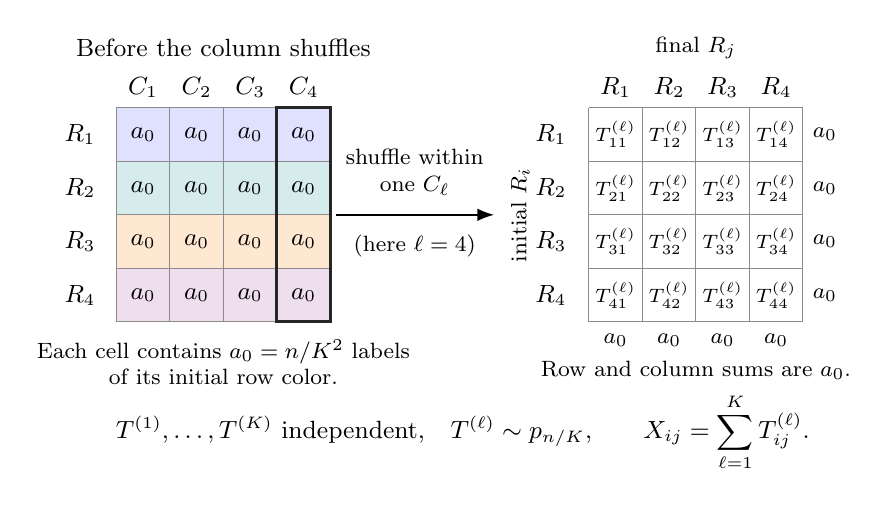
\begin{tikzpicture}[
  x=1cm,y=1cm,>=Latex,
  every node/.style={font=\small},
  gridline/.style={draw=black!45,line width=.35pt},
  tableentry/.style={font=\scriptsize},
  note/.style={font=\footnotesize}
]
  \foreach \row/\tone in {1/blue!12,2/teal!16,3/orange!18,4/violet!13} {
    \pgfmathsetmacro{\yb}{(4-\row)*.68}
    \fill[\tone] (0,\yb) rectangle (2.72,\yb+.68);
    \node[anchor=east] at (-.14,\yb+.34) {$R_{\row}$};
    \foreach \col in {1,...,4} {
      \pgfmathsetmacro{\xc}{(\col-.5)*.68}
      \node at (\xc,\yb+.34) {$a_0$};
    }
  }
  \foreach \line in {0,...,4} {
    \draw[gridline] (\line*.68,0)--(\line*.68,2.72);
    \draw[gridline] (0,\line*.68)--(2.72,\line*.68);
  }
  \foreach \col in {1,...,4} {
    \node at ({(\col-.5)*.68},2.98) {$C_{\col}$};
  }
  \draw[black!85,line width=1.1pt] (2.04,0) rectangle (2.72,2.72);
  \node at (1.36,3.48) {Before the column shuffles};
  \node[note,align=center] at (1.36,-.51)
    {Each cell contains $a_0=n/K^2$ labels\\of its initial row color.};

  \draw[->,line width=.7pt] (2.79,1.36)--(4.80,1.36);
  \node[note,align=center] at (3.79,1.90) {shuffle within\\one $C_\ell$};
  \node[note] at (3.79,.97) {(here $\ell=4$)};

  \foreach \row in {1,...,4} {
    \pgfmathsetmacro{\yb}{(4-\row)*.68}
    \node[anchor=east] at (5.84,\yb+.34) {$R_{\row}$};
    \foreach \col in {1,...,4} {
      \pgfmathsetmacro{\xc}{6.00+(\col-.5)*.68}
      \node[tableentry] at (\xc,\yb+.34) {$T^{(\ell)}_{\row\col}$};
    }
    \node[note] at (9.00,\yb+.34) {$a_0$};
  }
  \foreach \line in {0,...,4} {
    \draw[gridline] (6.00+\line*.68,0)--(6.00+\line*.68,2.72);
    \draw[gridline] (6.00,\line*.68)--(8.72,\line*.68);
  }
  \foreach \col in {1,...,4} {
    \node at ({6.00+(\col-.5)*.68},2.98) {$R_{\col}$};
    \node[note] at ({6.00+(\col-.5)*.68},-.23) {$a_0$};
  }
  \node[rotate=90,note] at (5.13,1.36) {initial $R_i$};
  \node[note] at (7.36,3.48) {final $R_j$};
  \node[note] at (7.36,-.62) {Row and column sums are $a_0$.};

  \node[align=center] at (4.40,-1.40)
    {$T^{(1)},\ldots,T^{(K)}$ independent,\quad
      $T^{(\ell)}\sim p_{n/K}$,\qquad
      $X_{ij}=\displaystyle\sum_{\ell=1}^{K}T^{(\ell)}_{ij}$.};
\end{tikzpicture}
\caption{The middle round in the row--column--row construction
(schematic $K=4$; the proof uses $K=8$).
Every $C_\ell$ contains $a_0$ labels from each initial $R_i$ and $a_0$ slots
in each final $R_j$. Independent column shuffles produce the tables
$T^{(\ell)}$; their columns index final $R_j$ groups.
The first and last row shuffles supply right and left invariance,
respectively, making the permutation law uniform conditional on its count matrix.}
\label{fig:overlay-grid}
\end{figure}

Here is the comparison of this sum with \(p_n\). We may assume \(n\) is divisible by \(K^3\). Use as free coordinates the upper-left \((K-1)\times(K-1)\) subtable, treated as a vector of size \(b=(K-1)^2\). For \(M\) divisible by \(K^2\) and \(X\sim p_M\), center the vector at its coordinate mean \(M/K^2\) and divide by \(\sqrt M\); call the result \(Z_M\). Let \(J\) be the linear map completing a free-coordinate vector to a full matrix with zero row and column sums. Uniformly for \(\|z\|\) bounded on the centered scaled lattice,
\begin{equation}
 \Pr(Z_M=z)=M^{-b/2}
   \left(G(z)+o(1)\right),\qquad
 G(z)=c_K \exp\!\left(-K^2\|J z\|^2/2\right),                           \label{special:overlay:eq:7}
\end{equation}
where matrix norm here is Euclidean and \(c_K>0\) depends only on \(K\). To see this, substitute \(x_{ij}=a+\sqrt M (Jz)_{ij}\) with \(a=M/K^2\) in \eqref{special:overlay:eq:6} (nonnegativity holds for bounded \(z\) and large \(M\)). Stirling's formula and expansion of \(x\log x-x\) about \(a\) have canceling linear terms in the sum. The constant terms cancel with the numerator and \(M!\) and the quadratic terms give \(K^2\|Jz\|^2/2\), with remainders \(o(1)\) for bounded \(z\). The square-root factors give \(M^{K-1/2-K^2/2}=M^{-b/2}\) times a constant \((2\pi)^{-b/2}K^{K^2-K}\) and \(1+o(1)\), proving \eqref{special:overlay:eq:7}.

Writing \(W\) for an independent uniform vector on \([0,1)^b\), \(Z_M+W/\sqrt M\) has density converging in \(L^1\) to \(G\). On compacts this follows from \eqref{special:overlay:eq:7} and continuity. Tail probabilities are uniformly small on taking large compacts since each count coordinate is hypergeometric with variance at most \(M\); the limit density is integrable since \(J\) is injective. This proves the \(L^1\) convergence and in particular normalization, so \(G\) is a centered nondegenerate Gaussian density.

For the sum of \(K\) tables from \(p_{n/K}\), the centered vector at scale \(1/\sqrt n\) is a sum of \(K\) independent \(Z_{n/K}/\sqrt K\). First add independent noise \(W_i/\sqrt n\) to each summand. By the density convergence, independence and total-variation contraction under addition, the noisy sum converges in total variation to the law with density \(G\): the sum of \(K\) centered Gaussians of this law each divided by \(\sqrt K\) has the same law. This convergence still holds keeping only the noise on the first summand. Indeed that smoothed summand by itself converges in total variation to a Gaussian (scaled by \(1/\sqrt K\)). Its distance to its translate by any vector of norm at most \((K-1)\sqrt b/\sqrt n\) therefore tends to zero uniformly, by continuity of translations of the Gaussian density in \(L^1\). Conditioning on the other summands and their noises bounds by this \(o(1)\) the distance induced by removing their noises. Thus, with a single noise, both the centered scaled sum and the \(p_n\) vector are close to the same law by \eqref{special:overlay:eq:7} and the sum argument. Total variation between these two noisy laws equals the discrete total variation without noise since both lattices have the same cells spread out uniformly by the noise. This proves the desired count-law comparison, hence mixing of the ideal product.
\end{proof}

\label{special:overlay:bound}
We conclude that the overlay product conditional on the base has expected total-variation distance \(o(1)\) from a uniform permutation on \(V\). Multiplying by the final base permutation (fixed under the conditioning) preserves the comparison with uniform. Removing the conditioning and mapping back to the deck locations proves total-variation distance \(o(1)\) for the actual shuffle. All estimates hold for any initial deck by identifying its cards with their starting positions. The shuffle has uniform stationary law since every layer applies a random permutation according to switches independent of the incoming deck. We used \(3K\cdot k\cdot 21d\) full layers of the type counted as steps in the shuffle definition. This gives the upper bound by an absolute multiple of \(d\) for sufficiently large \(d\).
The choices give $\delta=1/16384$, $k=65536$, and $3Kk\cdot21=33030144$, so the upper time is $33030144d$ complete shuffles.

This proves Theorem~\ref{thm:overlay}. The support bound of Section~\ref{sec:conditional} also gives $t_{\mathrm{mix}}\ge d$ for all sufficiently large $d$.

\section{Two independent half-permutations}\label{sec:two-halves}

The previous constructions extract contraction from repeated active intervals. This construction uses two long independent blocks. For the second block, reveal only which slots contain each of two colors at every layer. That observation leaves independent internal permutations of the two colors. We will trim their large tuple marginals and combine them with inverse-image information from the first block. The two orientations have different roles and must both be retained.

\subsection{The two precise inputs}

Here we use two companion results. We state their full hypotheses so that the conditional law to which each applies is explicit. Write $\operatorname{inj}(I,J)$ for the set of injections from a finite ordered set $I$ into a finite set $J$.

The conditional path theorem~\cite[Theorem~4.1]{conditional-information} has the following form. Fix $0<p<1$ and define
\begin{equation}\label{eq:tabloid-parameters}
 \rho_p=\frac{3+p}{4},\qquad c_p=-\frac18\log_2\rho_p,
 \qquad b=\lceil10/c_p\rceil.
\end{equation}
For every deterministic starting deck, every specified base set of $r_0$ labels, and every ordered list of $k$ additional labels satisfying $r_0+k-1\le pn$, after $2b$ sweeps,
\begin{equation}\label{eq:conditional-input}
 \E_{\mathcal H}\left\|
 \mathcal L(\text{list endpoints}\mid\mathcal H)
 -\operatorname{Unif}\operatorname{inj}([k],V\setminus E_{\mathcal H})
 \right\|_{\TV}\le k n^{-4}.
\end{equation}
Here $\mathcal H$ is the full labelled base-path history and $E_{\mathcal H}$ its endpoint set. The estimate holds for every cyclic coordinate order, including the reverse order. It also holds after coarsening $\mathcal H$, provided the endpoint available set remains determined. All thresholds depend only on the fixed $p$.

The abstract conditional-product transfer~\cite[Theorem ``Conditional-product transfer'']{partial-fourier} concerns $V=A\sqcup C$ with $|A|=|C|=h$, and $H=S_A\times S_C$. Partition each half into $L$ equal buffers, where $L\ge2C_0$ and $C_0=2000000$. Suppose a subprobability $\xi$ on $S_V$ has both ordered inverse-image marginals $x^{-1}|_A$ and $x^{-1}|_C$ pointwise at most twice uniform. For every environment $z$, let $\nu_A^z,\nu_C^z$ be subprobabilities on the two half-groups. Assume that, in each factor and for every buffer, the ordered image tuple on the complement of that buffer has marginal at most twice uniform. For each $z$, choose an arbitrary deterministic permutation $t_z\in S_V$. If $Z$ has any probability law, put
\[
 \omega=\E_Z\big[\delta_{t_Z}*(\nu_A^Z\otimes\nu_C^Z)\big],
 \qquad \theta=\omega*\xi.
\]
Then, for all sufficiently large $h$, every irreducible representation of $S_V$ of degree $D>1$ satisfies
\begin{equation}\label{eq:tabloid-transfer}
 \|\widehat\theta\|_{\op}\le\sqrt{22}\,D^{-1/40}.
\end{equation}
The Hilbert--Schmidt norms in that theorem use ordinary, unnormalized trace. For either $J\in\{A,C\}$, let $\nu_J$ be a factor satisfying the buffer caps and let $\gamma$ be an irreducible representation of $S_J$, of degree $D_\gamma$. The underlying buffer estimate is
$\|\widehat\nu_J(\gamma)\|_{\HS}^2/D_\gamma\le\min(1,2D_\gamma^{-1/2})$.
For irreducibles $\alpha$ of $S_A$, $\beta$ of $S_C$, and $\lambda$ of $S_V$, write $c_{\alpha\beta}^{\lambda}$ for the multiplicity of $\alpha\otimes\beta$ in the restriction of $\lambda$ to $H$. These multiplicities are retained through the estimate
$c_{\alpha\beta}^{\lambda}\le\min(D_\alpha,D_\beta)$, where each $D$ denotes the corresponding degree.
For the final Fourier sum we will use the local reciprocal-square estimate in Lemma~\ref{lem:degree-sum}.

These are separate inputs. The first supplies conditional tuple information from the shuffle; the second converts explicit caps and a conditional product into an operator bound. The product property will now be proved for the actual shuffle environment.

\subsection{Inverse-image caps for the first block}

\begin{theorem}[Two-half construction]\label{thm:two-halves}
Set $L=2^{23}$, $p=1-1/(2L)$, and choose $b$ by~\eqref{eq:tabloid-parameters}. For $n=2^d$, the full-deck law from any deterministic start approaches uniform in total variation after $400bd$ physical shuffles.
\end{theorem}

For these choices, $L$ divides $h=n/2$ for all sufficiently large $d$. Fix two halves $A,C$ of $V$ and partition each into $L$ buffers of size $h/L$. Let $X,W$ be independent permutations each generated by $2b$ forward sweeps, and let $\mu$ be the law of $WX$.

The inverse of $X$ is generated by the independent involutive layers in reverse order. Apply~\eqref{eq:conditional-input} with empty base and a list consisting of $A$, and then of $C$. Since $h-1\le pn$, each ordered inverse-image half-tuple has distance at most $h n^{-4}$ from uniform.

We use the following elementary truncation rule repeatedly. If probability laws $P,Q$ are on one finite set, then
\[
 P\{v:P(v)>2Q(v)\}\le2\|P-Q\|_{\TV},
\]
since $P(v)\le2(P(v)-Q(v))$ on those atoms and the total positive excess is the variation distance. Delete from the law of $X$ every permutation whose inverse-image tuple on either half is an atom of more than twice its uniform probability. Call the resulting subprobability $\xi$. It obeys both required pointwise caps, and
\begin{equation}\label{eq:x-mass}
 1-\xi(S_n)\le4h n^{-4}=2n^{-3}.
\end{equation}
The deletion for the other half cannot increase a marginal. Thus one common $\xi$ has the two caps simultaneously.

\subsection{The occupancy environment and the conditional product}

Color the positions at the start of $W$ by membership in $A$ or $C$, regarding those starting positions as distinct labels for this block. Let $Z$ record the set of positions occupied by each color after every layer, including the initial and final boundary. It records no labels within a color.

\begin{lemma}[Independent internal permutations]\label{lem:color-product}
For every feasible occupancy history $Z=z$, all mixed-color switch values are fixed and all same-color switch values are independent fair bits. Choose $t_z$ to send the increasing list of $A$ to the increasing list of its endpoint color set and likewise for $C$. Then
\[
 W=t_z(Y_A\times Y_C),
\]
where, conditional on $Z=z$, $Y_A\in S_A$ and $Y_C\in S_C$ are independent. Their conditional laws depend only on $z$.
\end{lemma}
\begin{proof}
At a mixed-color edge, the next pair of colors determines whether its coin is zero or one. At a same-color edge, either coin gives the same outgoing colors. Conversely, once the coins specified at the mixed edges of $z$ are fixed, induction on layers forces precisely the occupancy history $z$, independently of all same-color coins. Thus the event $Z=z$ is a cylinder in the time-edge array. Its unprescribed bits remain mutually independent.

A label of color $A$ uses fixed transports at mixed edges and only the independent bits on $A$--$A$ edges otherwise. The analogous assertion for color $C$ uses the disjoint array on $C$--$C$ edges. For fixed $z$ those two sets of time-edge coordinates are deterministic. Applying the slot-bijection construction separately to the two colors gives bijections onto their endpoint sets. The stated $t_z$ identifies these sets with the original halves, giving the independent permutations $Y_A,Y_C$. In particular no independence of the color history itself from the internal permutations is being used.
\end{proof}

Write $\mu_A^z,\mu_C^z$ for these two conditional probabilities. Fix a buffer $B\subset A$. Apply~\eqref{eq:conditional-input} to $W$ with all $C$ labels as base and the list $A\setminus B$ as the additional labels. Here
\[
 r_0+k-1=h+(h-h/L)-1
        =n-\frac n{2L}-1\le pn.
\]
The error is at most $(h-h/L)n^{-4}$. The full labelled $C$ paths determine the color occupancy history $Z$, and $Z$ still determines their endpoint set. Hence the allowed coarsening in~\eqref{eq:conditional-input} gives that same expected error conditional on $Z$. Applying the deterministic bijection $t_Z^{-1}$ sends the comparison law to uniform ordered distinct images in $A$. We conclude
\begin{equation}\label{eq:color-buffer-error}
 \E_Z\left\| (\mu_A^Z)_{A\setminus B}
          -(U_A)_{A\setminus B}\right\|_{\TV}
 \le(h-h/L)n^{-4}.
\end{equation}
The same argument applies to every buffer of $C$, interchanging the colors. The endpoints' available set is essential here: ordinary unconditional list mixing would not imply~\eqref{eq:color-buffer-error}.

For each $z$, delete from $\mu_J^z$ all permutations whose ordered image tuple outside any buffer exceeds twice its uniform probability, for $J=A,C$. Denote the subprobabilities by $\nu_J^z$ and their masses by $a_J(z)$. The truncation rule and~\eqref{eq:color-buffer-error} give
\[
 \E_Z\big[(1-a_A(Z))+(1-a_C(Z))\big]
 \le4L(h-h/L)n^{-4}=(2L-2)n^{-3}.
\]
Every surviving factor satisfies each cap for its particular $z$, even if the loss at that environment is large. Lemma~\ref{lem:color-product} now permits the product of these two deletions: define
\[
 \omega=\E_Z[\delta_{t_Z}*(\nu_A^Z\otimes\nu_C^Z)].
\]
It is dominated pointwise by the true law of $W$. Its missing mass is
$\E[1-a_Aa_C]$, bounded by the preceding display because
$1-a_Aa_C\le(1-a_A)+(1-a_C)$.

We have now established every conditional-law hypothesis of the transfer: the environment has its original probability law, each conditional measure is an actual product, each factor has all its buffer-complement caps, and the first block has the two inverse-image caps. Define $\theta=\omega*\xi$. Independence of the original blocks and positivity of convolution give $\theta\le\mu$ pointwise, while
\begin{equation}\label{eq:tabloid-mass}
 1-\theta(S_n)\le2L n^{-3}=o(1).
\end{equation}
The integer $L$ is large but fixed before $d$ tends to infinity.

\subsection{Fourier completion and physical time}

Applying~\eqref{eq:tabloid-transfer} gives the degree-power operator bound for every $D_\lambda>1$. We include the final deduction to keep the mass, parity and time conventions visible in this application.

The original block law $\mu$ has expected sign zero. Indeed, condition on all switch coins except any one coin in a physical layer. Flipping that fair coin composes the final permutation with a conjugate transposition and reverses its sign. From $\theta\le\mu$ and~\eqref{eq:tabloid-mass},
\[
 |\widehat\theta(\sgn)|\le1-\theta(S_n)\le2L n^{-3}.
\]
Let $j=100$ and $q=\theta(S_n)$. The trivial Fourier coefficient of
$\theta^{*j}-U_n$ is $q^j-1=o(1)$ and its sign coefficient is
$\widehat\theta(\sgn)^j=o(1)$. For all other irreducibles, without assuming their matrices commute or are normal,
\[
 \sum_{D_\lambda>1}D_\lambda
       \|\widehat\theta(\lambda)^j\|_{\HS}^2
 \le22^j\sum_{D_\lambda>1}D_\lambda^{2-2j/40}
 =22^{100}\sum_{D_\lambda>1}D_\lambda^{-3}=o(1).
\]
We used submultiplicativity of the operator norm,
$\|B\|_{\HS}^2\le D\|B\|_{\op}^2$, and Lemma~\ref{lem:degree-sum}, since $D^{-3}\le D^{-2}$.
Plancherel and Cauchy--Schwarz imply
$\|\theta^{*100}-U_n\|_1=o(1)$. Restoring the missing measure costs
$1-q^{100}=o(1)$, so $\|\mu^{*100}-U_n\|_{\TV}\to0$.

Each of $X,W$ costs $2bd$ physical shuffles. One macro-step therefore costs $4bd$, and the $100$ independent macro-steps cost $400bd$. They concatenate at sweep boundaries and hence have exactly the physical shuffle law at that time. Translation by any fixed initial deck preserves total variation. This proves Theorem~\ref{thm:two-halves}.

\begin{thebibliography}{99}

\bibitem{bbl2009}
J. Borcea, P. Br\"and\'en, and T. M. Liggett,
Negative dependence and the geometry of polynomials,
\emph{Journal of the American Mathematical Society} \textbf{22} (2009), no.~2, 521--567.
\href{https://doi.org/10.1090/S0894-0347-08-00618-8}{doi:10.1090/S0894-0347-08-00618-8}.

\bibitem{czumaj-vocking2014}
A.~Czumaj and B.~V\"ocking,
Thorp shuffling, butterflies, and non-Markovian couplings,
\emph{Automata, Languages, and Programming---ICALP 2014},
Lecture Notes in Computer Science, vol.~8572, Springer, 2014,
344--355.
\href{https://doi.org/10.1007/978-3-662-43948-7_29}
{doi:10.1007/978-3-662-43948-7\_29}.

\bibitem{etingof}
P.~Etingof, O.~Golberg, S.~Hensel, T.~Liu, A.~Schwendner,
D.~Vaintrob, and E.~Yudovina,
\emph{Introduction to Representation Theory},
Student Mathematical Library, vol.~59, American Mathematical Society,
2011.
Author's lecture-note version, January 10, 2011:
\url{https://math.mit.edu/~etingof/replect.pdf}.

\bibitem{hastad2006}
J.~H\aa stad,
The square lattice shuffle,
\emph{Random Structures \& Algorithms} \textbf{29} (2006), no.~4,
466--474.
\href{https://doi.org/10.1002/rsa.20131}{doi:10.1002/rsa.20131}.
Correction: \textbf{48} (2016), no.~1, 213,
\href{https://doi.org/10.1002/rsa.20620}{doi:10.1002/rsa.20620}.
Author texts:
\url{https://www.csc.kth.se/~johanh/jhsquare.pdf} (October 20, 2005)
and \url{https://johanhastad.se/nntypo.pdf} (June 17, 2015).

\bibitem{hmr2014}
V. T. Hoang, B. Morris, and P. Rogaway,
\emph{An enciphering scheme based on a card shuffle},
Advances in Cryptology---CRYPTO 2012,
Lecture Notes in Computer Science 7417, Springer, 2012, 1--13.
The cited Section 3, Theorem 3, and Lemma 4 refer to
\href{https://arxiv.org/abs/1208.1176v2}{arXiv:1208.1176v2},
21 November 2014.

\bibitem{keller-lifshitz-sheinfeld2024}
N. Keller, N. Lifshitz, and O. Sheinfeld,
\emph{Improved covering results for conjugacy classes of symmetric groups
via hypercontractivity},
Forum of Mathematics, Sigma 12 (2024), e85, 1--19,
\href{https://doi.org/10.1017/fms.2024.95}{doi:10.1017/fms.2024.95}.
Definition 2.1 and Theorem 2.2 give the orbit-growth parameter and
the uniform fixed-slack formulation of the Larsen--Shalev bound.

\bibitem{larsen-shalev2008}
M. Larsen and A. Shalev,
\emph{Characters of symmetric groups: sharp bounds and applications},
Inventiones Mathematicae 174 (2008), no.~3, 645--687,
\href{https://doi.org/10.1007/s00222-008-0145-7}{doi:10.1007/s00222-008-0145-7}.

\bibitem{liebeck-shalev2004}
M. W. Liebeck and A. Shalev,
\emph{Fuchsian groups, coverings of Riemann surfaces, subgroup growth,
random quotients and random walks},
Journal of Algebra 276 (2004), no.~2, 552--601.
The cited Proposition 2.5 and Theorem 2.6 appear on pages 15--16
of the \href{https://www.ma.ic.ac.uk/~mwl/fuchs.pdf}{author's text}.

\bibitem{montenegro-tetali2006}
R. Montenegro and P. Tetali,
\emph{Mathematical aspects of mixing times in Markov chains},
Foundations and Trends in Theoretical Computer Science 1 (2006), no.~3,
237--354, \href{https://doi.org/10.1561/0400000003}{doi:10.1561/0400000003}.

\bibitem{morris44}
B.~Morris,
The mixing time of the Thorp shuffle,
\emph{SIAM Journal on Computing} \textbf{38} (2008), no.~2, 484--504.
\href{https://doi.org/10.1137/050636231}{doi:10.1137/050636231}.
Preprint: \url{https://arxiv.org/abs/math/0507307v1}.

\bibitem{morris-exclusion2006}
B.~Morris,
The mixing time for simple exclusion,
\emph{Annals of Applied Probability} \textbf{16} (2006), no.~2,
615--635.
\href{https://doi.org/10.1214/105051605000000728}
{doi:10.1214/105051605000000728}.
Lemma~12 is cited from the IMS electronic reprint
\href{https://arxiv.org/abs/math/0405157v2}{arXiv:math/0405157v2},
July 12, 2006, Section~5.3, pp.~19--20; its pagination differs
from the journal.

\bibitem{morris4}
B.~Morris,
Improved mixing time bounds for the Thorp shuffle and $L$-reversal chain,
\emph{Annals of Probability} \textbf{37} (2009), no.~2, 453--477.
\href{https://doi.org/10.1214/08-AOP409}{doi:10.1214/08-AOP409}.
Preprint: \url{https://arxiv.org/abs/0802.0339}.

\bibitem{morris3}
B.~Morris,
Improved mixing time bounds for the Thorp shuffle,
\emph{Combinatorics, Probability and Computing} \textbf{22} (2013),
no.~1, 118--132.
\href{https://doi.org/10.1017/S0963548312000478}
{doi:10.1017/S0963548312000478}.
Preprint: \url{https://arxiv.org/abs/0912.2759}.

\bibitem{mrs}
B. Morris, P. Rogaway, and T. Stegers,
\emph{How to encipher messages on a small domain:
deterministic encryption and the Thorp shuffle},
Advances in Cryptology---CRYPTO 2009,
Lecture Notes in Computer Science 5677, Springer, 2009, 286--302,
\href{https://doi.org/10.1007/978-3-642-03356-8_17}{doi:10.1007/978-3-642-03356-8\_17}.
Theorem 1 and Lemma 2 (proved in Appendix A) are cited from the
\href{https://www.cs.ucdavis.edu/~rogaway/papers/thorp.pdf}{author's conference text}.
A later journal version is \emph{Deterministic encryption with the Thorp shuffle},
Journal of Cryptology 31 (2018), no.~2, 521--536,
\href{https://doi.org/10.1007/s00145-017-9262-z}{doi:10.1007/s00145-017-9262-z}.

\bibitem{nummelin1978}
E. Nummelin,
A splitting technique for Harris recurrent Markov chains,
\emph{Zeitschrift f\"ur Wahrscheinlichkeitstheorie und Verwandte Gebiete}
\textbf{43} (1978), 309--318.
\href{https://doi.org/10.1007/BF00534764}{doi:10.1007/BF00534764}.

\bibitem{conditional-sweeps}
OpenAI,
\emph{Conditional coordinate sweeps and analytic transfer},
OpenAI Math Release preprint
\href{https://github.com/openai/math/blob/main/preprints/Conditional-coordinate-sweeps-and-analytic-transfer-September-26-2026/main.pdf}{OAI:Conditional-coordinate-sweeps-and-analytic-transfer-September-26-2026},
2026.

\bibitem{conditional-information}
OpenAI,
\emph{Conditional information under deterministic coordinate sweeps},
OpenAI Math Release preprint
\href{https://github.com/openai/math/blob/main/preprints/Conditional-information-under-deterministic-coordinate-sweeps-September-26-2026/main.pdf}{OAI:Conditional-information-under-deterministic-coordinate-sweeps-September-26-2026},
2026.

\bibitem{partial-fourier}
OpenAI,
\emph{From partial permutation information to Fourier bounds},
OpenAI Math Release preprint
\href{https://github.com/openai/math/blob/main/preprints/From-partial-permutation-information-to-Fourier-bounds-September-26-2026/main.pdf}{OAI:From-partial-permutation-information-to-Fourier-bounds-September-26-2026},
2026.

\bibitem{optimal-order}
OpenAI,
\emph{Optimal-order mixing of the Thorp shuffle},
OpenAI Math Release preprint
\href{https://github.com/openai/math/blob/main/preprints/Optimal-order-mixing-of-the-Thorp-shuffle-September-26-2026/paper.pdf}{OAI:Optimal-order-mixing-of-the-Thorp-shuffle-September-26-2026},
2026.

\bibitem{random-frames}
OpenAI,
\emph{Random coordinate frames and partial permutation laws},
OpenAI Math Release preprint
\href{https://github.com/openai/math/blob/main/preprints/Random-coordinate-frames-and-partial-permutation-laws-September-26-2026/main.pdf}{OAI:Random-coordinate-frames-and-partial-permutation-laws-September-26-2026},
2026.

\bibitem{sagan}
B.~E.~Sagan,
\emph{The Symmetric Group: Representations, Combinatorial Algorithms,
and Symmetric Functions}, second edition,
Graduate Texts in Mathematics, vol.~203, Springer, 2001.
\href{https://doi.org/10.1007/978-1-4757-6804-6}
{doi:10.1007/978-1-4757-6804-6}.

\bibitem{thorp}
E.~O.~Thorp,
Nonrandom shuffling with applications to the game of Faro,
\emph{Journal of the American Statistical Association} \textbf{68}
(1973), no.~344, 842--847.
\href{https://doi.org/10.1080/01621459.1973.10481434}
{doi:10.1080/01621459.1973.10481434}.

\end{thebibliography}

\end{document}
